\part{Start-up}
\chapter{Start-up e impresa}
Eric Ries, creatore della metodologia Lean Startup, definisce la start-up come
\begin{center}
\textit{“una istituzione umana nata per creare un nuovo prodotto o servizio in condizioni di estrema incertezza”}    
\end{center}
Paul Graham la descrive come
\begin{center}
\textit{"una istituzione concepita per crescere in maniera rapida”}
\end{center}
mentre Steve Blank la vede come 
\begin{center}
\textit{"un organizzazione temporanea che ha lo scopo di cercare un business model che abbia le seguenti caratteristiche: scalabile, replicabile, sostenibile e attuabile"}
\end{center}
\begin{redbar}
La migliore definizione di \textbf{start-up}\index{Start-up} è quella che comprende le tre precedenti, quindi, può essere descritta come un’azienda giovane e innovativa, orientata alla crescita rapida e capace di adattarsi e replicarsi in contesti sempre più ampi.
\end{redbar}
La principale differenza tra una start-up e un’impresa tradizionale sta nell'obiettivo di crescita. Un’impresa ordinaria, come un ristorante o una palestra, non è progettata per una crescita scalabile; in genere, essa punta a soddisfare una domanda esistente e a generare profitto stabile. Al contrario, una start-up nasce con un progetto innovativo e scalabile, ovvero che mira a sconvolgere il mercato e può crescere in modo esponenziale, trasformandosi rapidamente in una grande impresa.

In altri termini la start-up innovativa nasce con l’intento di stupire il mercato con una nuova idea che potrebbe cambiare la vita delle persone o di un determinato settore di mercato. Un’ impresa, invece, nasce quasi sempre con l’obiettivo principale di generare profitto.

\section{Crescita di una start-up}
Il percorso di crescita di una start-up segue un andamento a "\textit{hockey stick}"\index{Start-up!hockey stick} (bastone da hockey), caratterizzato da una fase iniziale di crescita lenta o stagnante, seguita da una rapida impennata (Figura \ref{fig:hockey-stick-growth}). Questa crescita si articola in quattro fasi:

\begin{figure}[ht]
    \centering
    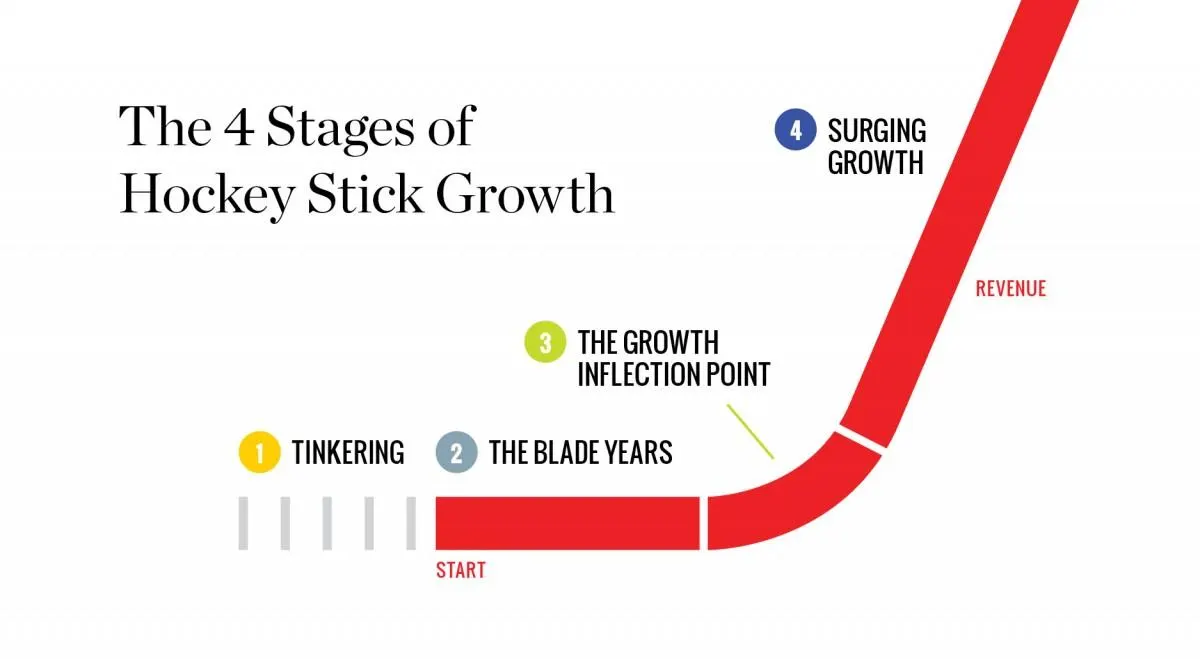
\includegraphics[width=0.65\linewidth]{images/hockey-stick-growth.png}
    \caption{Crescita a mazza da hockey}
    \label{fig:hockey-stick-growth}
\end{figure}

\begin{enumerate}
    \item \textit{Tinkering Stage.} Rappresenta il momento in cui gli imprenditori iniziano a esplorare e valutare la propria idea di start-up con maggiore serietà. In questo stadio, la priorità è comprendere se l'idea possa realmente funzionare nel mercato e individuare un equilibrio tra il problema da risolvere e la soluzione offerta. È un momento delicato in cui gli imprenditori cercano di sviluppare un prodotto o un servizio che risponda a una necessità reale, senza però fare il passo definitivo di trasformare l’idea in un’attività commerciale a pieno titolo.

    Durante il tinkering stage, i fondatori di solito non abbandonano il loro impiego principale e lavorano all’idea di start-up come progetto parallelo. Nonostante l’apparente bassa pressione, vi sono errori comuni che possono mettere a rischio la riuscita dell'idea. Uno di questi è l’eccessivo tempo dedicato alla costruzione di un complesso modello di business, che in questa fase iniziale rischia di allontanare i fondatori dalla sperimentazione pratica. Un altro errore frequente è la mancata condivisione di prototipi o modelli con potenziali clienti per raccogliere feedback. Spesso, infatti, la paura che i concorrenti possano copiare l’idea frena gli imprenditori dal ricevere critiche costruttive che permetterebbero di perfezionare il prodotto. La sperimentazione e lo sviluppo, basati sui commenti ricevuti dai potenziali utenti, dovrebbero essere il fulcro dell’attività durante questa fase.

    \item \textit{Blade Years Stage.} L’idea inizia a prendere forma e a essere convalidata sul mercato, in questo periodo, gli imprenditori sviluppano versioni preliminari del prodotto, come un MVP (Minimum Viable Product) o una versione beta, per testare la reazione del mercato e verificare la validità del modello di business. È il momento in cui i fondatori lasciano il loro lavoro principale per dedicarsi interamente alla start-up, segnando un punto di svolta nel livello di impegno e di rischio personale.

    Questa fase può durare dai tre ai quattro anni e, di solito, i ricavi sono limitati. Per coprire le spese, gli imprenditori spesso utilizzano fondi propri, pratica conosciuta come bootstrapping. Tuttavia, alcune insidie possono compromettere il successo della start-up anche in questo stadio. Spesso gli imprenditori, trovandosi senza entrate sufficienti per coprire le spese personali, concentrano i propri sforzi sulla preparazione di presentazioni elaborate per attirare investitori, un’attività che può essere dispendiosa in termini di tempo ed energie. In aggiunta, talvolta si verificano investimenti eccessivi in costose campagne di marketing e vendite, oppure un’eccessiva rigidità nei confronti del prodotto, che limita la capacità di adattarsi ai cambiamenti del mercato. La chiave di successo in questa fase è la flessibilità e l’apertura al miglioramento continuo.

    \item \textit{Growth Inflection Point.} Rappresenta il momento cruciale in cui il modello di business viene perfezionato e i ricavi iniziano a crescere rapidamente. Si tratta del “punto di svolta”, quando la start-up entra in una fase di crescita esponenziale e inizia a catturare l’interesse di venture capitalist e altri investitori. In questo stadio, la start-up acquisisce una notevole visibilità e attrattiva, diventando un’opportunità appetibile per chi è interessato a investire in progetti con alto potenziale di ritorno economico.

    Nonostante le opportunità offerte, questa fase presenta sfide significative. La crescita rapida può diventare insostenibile per alcune start-up, che rischiano di collassare sotto la pressione della domanda e delle nuove richieste del mercato. Alcuni imprenditori, attratti dal desiderio di sfruttare questa fase favorevole, apportano cambiamenti radicali a un modello di business che ha già dimostrato la sua validità. Tuttavia, l’attenzione principale dovrebbe essere rivolta a sincronizzare la gestione delle operazioni con l’aumento dei ricavi, mantenendo al contempo la stabilità del modello di business.

    \item \textit{Surging Growth Stage.} La start-up ha raggiunto una crescita sostenibile e può mantenere l’andamento esponenziale anche oltre il punto di inflezione. Questo stadio è caratterizzato da un’accelerazione continua, con una clientela in costante aumento. La gestione dell’azienda diventa più complessa, poiché l’aumento della domanda e l’attenzione del mercato generano nuove sfide, sia in termini di operatività sia di gestione strategica.

    In questo periodo, la start-up attira spesso offerte di acquisizione da parte di grandi aziende, interessate a integrare l’innovazione nel proprio modello di business. Gli imprenditori si trovano di fronte a una decisione strategica: vendere l’azienda, continuare a guidarla come amministratori delegati o assumere un CEO esterno per gestire la crescita. Indipendentemente dalla scelta, la transizione deve essere gestita con attenzione, reclutando manager di alta qualità e competenze per dirigere i dipartimenti principali. È essenziale evitare l’errore di affidare ruoli chiave a persone non qualificate, basandosi su relazioni personali piuttosto che sulle competenze professionali.
\end{enumerate}

\section{Esempi di crescita a "hockey stick"}
Il modello di crescita a “hockey stick” rappresenta l’evoluzione tipica delle start-up che riescono a superare con successo le fasi iniziali e a raggiungere una crescita rapida e sostenuta. Questo modello è stato esemplificato da diverse aziende, sia internazionali sia italiane, che sono riuscite a crescere rapidamente e a raggiungere traguardi straordinari.

\begin{Example}{Groupon}{}
Groupon è uno dei primi esempi di crescita a bastone da hockey. Fondata nel 2008 da Andre Mason ed Eric Lefkofsky come marketplace di e-commerce, l’azienda ha vissuto un percorso di crescita significativo che riflette le diverse fasi tipiche di questo modello.
\begin{enumerate}
    \item \textit{Tinkering.} Prima di diventare Groupon, Andrew Mason aveva lanciato nel 2006 “The Point”, un sito che puntava a creare un marketplace per gruppi di acquisto. Durante questa fase, che durò circa due anni, i ricavi furono molto bassi, attestandosi intorno ai 10.000 euro.
    \item \textit{The Blade Years.} Tra il 2008 e il 2010, Groupon ha attraversato un periodo di crescita stabile, ma non esplosiva, con entrate che raggiunsero i 14,5 milioni di euro.
    \item \textit{Growth Inflection Point.} Nel 2010 Groupon raggiunse il suo punto di inflezione, con ricavi che salirono a 313 milioni di euro.
    \item \textit{Surging Growth.} La fase di maturità per Groupon arrivò nel 2011, quando i ricavi superarono il miliardo di euro, segnando il successo dell’azienda a livello globale.
\end{enumerate}    
\end{Example}

\begin{Example}{Netflix}{}
Un altro esempio emblematico è Netflix, fondata nel 1997 da Reed Hastings come azienda di noleggio DVD. Netflix attraversò diverse fasi prima di diventare il colosso dello streaming che conosciamo oggi.
\begin{enumerate}
    \item \textit{Tinkering.} Dal 1996 al 1997, Netflix operava ancora come servizio di noleggio DVD.
    \item \textit{The Blade Years.} Tra il 1997 e il 2000, Netflix iniziò a crescere gradualmente, accumulando ricavi per circa 1,5 milioni di euro. Fu in questa fase che l’azienda abbandonò la vendita di DVD per concentrarsi sui servizi di abbonamento, una decisione che avrebbe poi permesso a Netflix di differenziarsi dai concorrenti.
    \item \textit{Growth Inflection Point.} Il 2000 rappresentò un anno di svolta per Netflix, con un fatturato di 41 milioni di euro e una base clienti in rapida espansione.
    \item \textit{Surging Growth.} Nel 2001, Netflix lanciò un’IPO (Offerta Pubblica Iniziale) a 15 dollari per azione e raggiunse circa 500.000 abbonati.
\end{enumerate}
\end{Example}

\begin{Example}{Yoox}{}
Anche in Italia troviamo esempi di start-up che hanno vissuto una crescita a bastone da hockey. Yoox, fondata nel 2000 da Federico Marchetti, divenne il primo “unicorno” italiano, ossia una start-up con una valutazione superiore a un miliardo di euro.
\begin{enumerate}
    \item \textit{Tinkering.} Tra il 1999 e il 2000, Yoox sperimentò il modello di e-commerce per la vendita di capi di abbigliamento off-season dei grandi marchi, cercando di posizionarsi come piattaforma innovativa nel settore della moda.
    \item \textit{The Blade Years.} Nei successivi due anni, Yoox iniziò a vendere a livello internazionale, raggiungendo un fatturato di circa 1,5 milioni di euro. Questa fase permise all’azienda di consolidare la sua presenza nel mercato e di iniziare a espandersi oltre i confini nazionali.
    \item \textit{Growth Inflection Point.} Il 2006 segnò il punto di inflessione della crescita di Yoox, con un fatturato di circa 70 milioni di euro. In questo periodo, Yoox sviluppò siti “powered by yoox” per grandi marchi della moda, che le permisero di aumentare ulteriormente la visibilità.
    \item \textit{Surging Growth.} Nel 2009, Yoox venne quotata al segmento STAR della Borsa Italiana con una valutazione di circa 217 milioni di euro. La crescita continuò fino alla fusione con Net-a-Porter nel 2015, creando YNAP, valutata 1,3 miliardi di euro. Nel 2018, il gruppo Richemont acquisì YNAP, al momento valutata 5,3 miliardi di euro.
\end{enumerate}
\end{Example}

\begin{Example}{Facile.it}{}
Un altro esempio di successo italiano è Facile.it, fondata nel 2008 da Alberto Genovese come comparatore di assicurazioni. L’azienda si evolse rapidamente, ampliando la propria offerta e consolidando la sua posizione nel mercato.
\begin{enumerate}
    \item \textit{Tinkering.} Tra il 2007 e il 2008, Facile.it operava come Assicurazione.it, focalizzandosi sulla comparazione delle polizze assicurative.
    \item \textit{The Blade Years.} Tra il 2008 e il 2010, Facile.it continuò a crescere stabilmente, raggiungendo un fatturato di 1,5 milioni di euro.
    \item \textit{Growth Inflection Point.} Nel 2011, Facile.it ampliò il proprio raggio d’azione alla comparazione di prodotti finanziari come mutui e prestiti, ricevendo anche un primo investimento significativo.
    \item \textit{Surging Growth.} La fase di maturità iniziò nel 2014, quando Oakley Capital entrò nella società, che continuò a triplicare i ricavi fino a raggiungere 106 milioni di euro nel 2019. Nel 2022, Facile.it fu acquisita da Silver Lake Partners, che la valutò oltre 1 miliardo di euro, confermando il suo status di unicorno.
\end{enumerate}
\end{Example}

\begin{Example}{Satispay}{}
Infine, Satispay rappresenta un esempio recente di crescita rapida nel settore dei pagamenti digitali. Fondata nel 2013 da Alberto Dalmasso, Dario Brignone e Samuele Pinta, Satispay ha introdotto una soluzione alternativa ai pagamenti con carta di credito e contante.
\begin{enumerate}
    \item \textit{Tinkering.} Tra il 2012 e il 2013, i fondatori testarono il concetto e iniziarono a raccogliere i primi fondi per avviare l’attività.
    \item \textit{The Blade Years.} Dal 2014 al 2017, Satispay ottenne i primi investimenti e registrò una crescita costante del numero di utenti.
    \item \textit{Growth Inflection Point.} Nel 2018, Satispay raggiunse i 500.000 utenti, consolidando la sua presenza nel settore dei pagamenti digitali.
    \item \textit{Surging Growth.} Dal 2020 in poi, la crescita esplose: nel 2022 Satispay raggiunse lo status di unicorno con un finanziamento di 320 milioni di euro. Oggi, con oltre 4 milioni di utenti e 300.000 esercizi commerciali convenzionati, Satispay continua a espandersi, con volumi di transazioni processate in costante aumento.
\end{enumerate}
\end{Example}

\chapter{Start-up in Italia}
In Italia, il concetto di \textit{start-up innovativa}\index{Start-up!start-up innovativa} è stato formalmente riconosciuto dall’ordinamento giuridico con il decreto-legge 179/2012, che ha introdotto una serie di norme specifiche per incoraggiare la creazione di imprese tecnologiche e innovative. Secondo il comma dell’articolo 25 di questo decreto
\begin{center}
\textit{"una start-up innovativa è definita come una società, inclusa anche in forma cooperativa, le cui azioni o quote rappresentative del capitale sociale non sono quotate su un mercato regolamentato o su un sistema multilaterale di negoziazione”, che possieda determinati requisiti analiticamente indicati dalla stessa norma e che, soprattutto, abbia come “oggetto sociale esclusivo o prevalente, lo sviluppo, la produzione e la commercializzazione di prodotti o servizi innovativi ad alto valore tecnologico."}    
\end{center}

\section{Start-up innovative}
Per essere considerata una start-up innovativa e beneficiare delle agevolazioni previste dalla legge, l’impresa deve soddisfare almeno uno dei seguenti requisiti:
\begin{enumerate}
    \item \textit{Investimento in ricerca e sviluppo.} La start-up deve destinare almeno il 15\% del maggiore tra il fatturato e i costi annui ad attività di ricerca e sviluppo.
    \item \textit{Forza lavoro qualificata.} Il team della start-up deve essere composto, per almeno un terzo, da dottorandi, dottori di ricerca o ricercatori, oppure per almeno due terzi da soci o collaboratori in possesso di una laurea magistrale.
    \item \textit{Brevetti e proprietà intellettuale.} La start-up deve essere titolare, depositaria o licenziataria di un brevetto registrato o di software protetto da copyright.
\end{enumerate}
Per incoraggiare gli investimenti nelle start-up innovative, il governo italiano ha introdotto agevolazioni fiscali per chi decide di investire in queste imprese. Le persone fisiche che investono nel capitale di una o più start-up o PMI innovative possono detrarre dalla propria dichiarazione dei redditi annuale un importo pari al 30\% dell’investimento, fino a un massimo di 1 milione di euro annui, con l’obbligo di mantenere l’investimento per almeno tre anni.

Allo stesso modo, anche le società che investono nel capitale di start-up innovative godono di una deduzione fiscale del 30\% sull’investimento effettuato, fino a un massimo di 1,8 milioni di euro all’anno. Anche in questo caso, l’investimento deve essere mantenuto per almeno tre anni. Queste agevolazioni hanno l’obiettivo di attrarre capitali verso le start-up, incentivando individui e aziende a sostenere lo sviluppo di nuove imprese innovative.

\chapter{Idea di business}
L'\textit{idea di business}\index{Start-up!idea di business} rappresenta il primo passo per avviare un'attività imprenditoriale. Per passare da un’intuizione a un progetto concreto, è necessario approfondire l’idea e darle una forma definita. Questo processo di sviluppo si compone di tre fasi principali: la fase di analisi, la fase creativa e la fase di maturazione e visione.

\section{Fase di analisi}
La \textit{fase di analisi} è il momento in cui si raccolgono informazioni e conoscenze sul mercato e sul settore in cui si desidera operare. L’obiettivo è stimolare il pensiero produttivo, cercando di scoprire opportunità innovative che potrebbero essere nascoste nei dati disponibili, ma che non sono ancora evidenti. Questo processo si basa sulla raccolta e sull'analisi di dati oggettivi, permettendo di fondare le fasi successive su una base solida e verificabile.

Uno dei metodi utilizzati per analizzare il mercato è la costruzione di una \textit{mappa dei trend}\index{Start-up!mappa dei trend}, che consente di individuare le tendenze attuali e future. La mappa dei trend parte dalla selezione del settore d’interesse, a cui segue la ricerca di parole chiave rilevanti (attraverso ricerche web, articoli scientifici e brevetti). I trend vengono poi classificati e organizzati all'interno della mappa, la quale viene aggiornata periodicamente per riflettere il grado di certezza dei trend identificati. Questa tecnica permette di visualizzare il contesto in cui l’idea di business potrebbe inserirsi e di individuare le aree di maggiore potenziale.

\section{Fase creativa}
La \textit{fase creativa} è caratterizzata dal pensiero produttivo, che include due abilità principali: il pensiero creativo e il pensiero critico. Il \textit{pensiero creativo} è essenziale per generare idee nuove e originali, spesso a partire da intuizioni spontanee o associazioni libere di pensieri. Tuttavia, queste idee sono spesso fragili e sfuggenti, per cui è importante dar loro spazio senza giudizio immediato, lasciando che si sviluppino liberamente. Questo tipo di pensiero è espansivo e permette la nascita di nuove idee a partire da altre già generate.

Dopo il pensiero creativo, è necessario adottare il \textit{pensiero critico}, che interviene per analizzare, valutare e selezionare le idee proposte, eliminando quelle meno efficaci e mantenendo solo le migliori. Questo processo di selezione è fondamentale per individuare le idee più solide, che possono essere trasformate in progetti concreti.

Un metodo spesso utilizzato nella fase creativa è il \textit{brainstorming}\index{Start-up!brainstorming}, una tecnica di generazione di idee sviluppata da Alex Osborn nel 1941. Il principio fondamentale del brainstorming è la separazione tra pensiero creativo e critico, che consente di generare idee senza vincoli di giudizio iniziale. Osborn riteneva infatti che un brainstorming efficace incoraggi la quantità e la diversità delle idee, creando combinazioni e miglioramenti tra le proposte dei partecipanti.

Un brainstorming produttivo si divide generalmente in tre fasi: nella prima si producono idee ordinarie, cui molti hanno già pensato. Nella seconda fase, le idee diventano più originali, con qualche intuizione insolita. Infine, nel terzo stadio, emergono le idee più innovative e dirompenti, quelle che costituiscono il “diamante” del brainstorming. Una volta raccolte le idee, si passa alla valutazione per identificare quelle che offrono maggior valore.

\section{Fase della maturazione e della visione}
Nella \textit{fase della maturazione e della visione}, l'idea viene affinata per far emergere tutti gli elementi necessari alla sua realizzazione e trasformazione in realtà. È in questo stadio che si valuta il potenziale di successo dell'idea, confrontandola con le aspettative del mercato e considerando aspetti pratici come la sostenibilità finanziaria e la scalabilità.

Per trasformare un’idea in una realtà imprenditoriale è fondamentale sviluppare un \textit{business model}, ovvero una struttura che identifichi il modo in cui l'azienda creerà, distribuirà e catturerà valore. Non tutte le idee, anche quelle apparentemente grandiose, si traducono in un successo; affinché l’idea abbia successo, deve rispondere a un bisogno concreto dei clienti, generare valore per loro e garantire una crescita rapida e sostenibile.

Per concretizzare un'idea di business in un modello pratico, le start-up spesso utilizzano il \textit{Business Model Canvas}, una metodologia grafica sviluppata da Alexander Osterwalder e Yves Pigneur. Questo strumento permette di visualizzare e organizzare gli elementi chiave necessari alla creazione di un business model di successo, favorendo la comprensione di aspetti quali il valore offerto, i segmenti di clientela, le risorse e le attività principali, i canali di distribuzione e le fonti di ricavo (Figura \ref{fig:business-model-canvas}).

Il business model canvas è diventato uno degli strumenti più usati non solo dalle start-up, ma anche dalle grandi aziende, per sviluppare nuovi prodotti o servizi innovativi. Rappresenta un metodo efficace per strutturare il proprio business model in modo semplice, ma completo, consentendo una rapida visione d’insieme e facilitando le decisioni strategiche.

\chapter{Business model}
\begin{redbar}
Il \textbf{business model}\index{Business model} (o modello di business) rappresenta l’insieme delle soluzioni organizzative e strategiche che un’impresa utilizza per acquisire un vantaggio competitivo nel mercato. Questo modello descrive il modo in cui un’azienda crea, distribuisce e cattura valore.    
\end{redbar}
Per una start-up, un business model efficace deve soddisfare quattro caratteristiche fondamentali:
\begin{enumerate}
    \item \textit{Sostenibilità.} Un modello di business sostenibile è in grado di produrre reddito, ovvero generare entrate superiori ai costi.
    \item \textit{Scalabilità.} La scalabilità indica la capacità del modello di crescere rapidamente e in modo esponenziale rispetto ai costi lineari.
    \item \textit{Replicabilità.} Per essere replicabile, un modello di business deve poter essere applicato in vari contesti e paesi, mantenendo la sua efficacia iniziale. Ciò significa che l’azienda può espandersi geograficamente e raggiungere nuovi mercati senza dover reinventare il proprio modello di business.
    \item \textit{Praticabilità.} Il modello di business deve essere realizzabile con le risorse e le tecnologie attuali. Ad esempio, un modello di business basato su una tecnologia futuristica come la “macchina del tempo” non sarebbe praticabile, poiché la tecnologia necessaria per costruirla non esiste.
\end{enumerate}
Una differenza importante esiste tra il business model e il business plan, due documenti spesso confusi ma che svolgono ruoli differenti. Il business model è una rappresentazione di come l’azienda creerà e catturerà valore, mentre il business plan è il documento che traduce il modello di business in una strategia operativa dettagliata. Il business plan, infatti, è un documento dettagliato che specifica "cosa", "quanto tempo" e "quanti soldi" sono necessari per realizzare il business model. Si tratta di un documento complesso e ricco di analisi e previsioni, fondamentale per ottenere finanziamenti, poiché è richiesto da stakeholder e investitori.

A differenza del business model, che offre una visione d’insieme di come l’azienda intende creare valore, il business plan è una vera e propria roadmap che definisce i passi operativi necessari per attuare il modello. Entrambi sono strumenti essenziali per una pianificazione efficace e dovrebbero essere usati in maniera complementare.

\section{Business model più diffusi}
Esistono diversi tipi di modelli di business, ognuno adatto a differenti settori e strategie di mercato. Tra i modelli più diffusi troviamo:
\begin{enumerate}
    \item \textit{Transazionale.} L’azienda vende un prodotto o servizio in cambio di un pagamento unico da parte del cliente.
    \item \textit{Marketplace.} Una piattaforma che mette in contatto venditori e acquirenti e ricava profitti dalle transazioni o dalle commissioni.
    \item \textit{Software as a Service (SaaS).} Il modello basato sulle iscrizioni, tipico delle aziende che offrono software in abbonamento.
    \item \textit{Freemium.} L’azienda offre un servizio base gratuito con opzioni a pagamento per funzionalità premium.
    \item \textit{Pay As You Go.} Il cliente paga solo per l’utilizzo effettivo del servizio.
    \item \textit{Noleggio o Leasing.} Modello in cui l’azienda concede in affitto prodotti a lungo termine.
    \item \textit{Franchising.} Un modello che consente a terzi di utilizzare il marchio e il modello di business dell’azienda in cambio di royalties.
    \item \textit{Broker.} Un intermediario che guadagna una commissione facilitando la compravendita tra due parti.
    \item \textit{Community.} Una piattaforma che riunisce una comunità di utenti e monetizza tramite pubblicità o iscrizioni.
    \item \textit{Affiliazione.} L’azienda guadagna commissioni promuovendo prodotti o servizi di terzi.
    \item \textit{Modello basato sulle inserzioni.} L’azienda genera ricavi dalle pubblicità.
    \item \textit{Donazione.} Modello di business senza scopo di lucro, sostenuto dalle donazioni volontarie.
\end{enumerate}

\subsection*{Transazionale}
Il \textit{modello transazionale} è uno dei modelli di business più tradizionali, utilizzato da aziende che puntano a generare ricavi attraverso la vendita diretta di prodotti o servizi ai consumatori. La logica alla base è semplice: l’azienda crea valore offrendo beni o servizi che rispondono alle necessità specifiche dei clienti, e i ricavi provengono direttamente dalle transazioni effettuate al momento degli acquisti. Questo tipo di modello si applica sia a contesti fisici, come negozi o punti vendita, sia a canali digitali, come gli e-commerce, garantendo una grande versatilità in diversi settori.

Uno dei principali punti di forza del modello transazionale è la flessibilità nella definizione dell’offerta, che permette all’azienda di personalizzare prodotti o servizi in base alle esigenze del mercato. Inoltre, le transazioni dirette favoriscono la creazione di relazioni forti con i clienti, elemento fondamentale per la fidelizzazione.

D’altro canto, il modello transazionale presenta alcune sfide significative. La creazione e il mantenimento di un brand forte richiedono un investimento considerevole di risorse, sia finanziarie che di tempo, e la gestione della catena del valore impone una strategia di marketing efficace e una gestione accurata dei flussi operativi. Nonostante queste difficoltà, l’adattabilità e la semplicità del modello transazionale lo rendono un’opzione ancora molto popolare.

\subsection*{Marketplace}
Il \textit{modello marketplace} si basa sulla creazione di una piattaforma che agisce come intermediario tra diversi gruppi di utenti, facilitando le transazioni e creando valore attraverso l’interconnessione. A differenza del modello transazionale, qui l’azienda non produce né possiede direttamente i beni o servizi scambiati. Al contrario, il suo ruolo è offrire l’infrastruttura e stabilire regole che permettono agli utenti di interagire in modo efficace.

Il valore aggiunto di questo modello risiede nella capacità della piattaforma di ridurre i costi di transazione, aumentare la trasparenza e incentivare gli scambi tra gli utenti, generando quello che viene definito effetto di rete. Questo effetto si verifica quando il valore della piattaforma cresce con l’aumentare del numero di partecipanti, rendendola progressivamente più attraente per nuovi utenti.

Il successo di un marketplace dipende in larga misura dalla capacità di attrarre e mantenere un numero sufficiente di utenti su entrambi i lati della piattaforma. Per fare ciò, le piattaforme di successo investono in sistemi di rating, meccanismi di risoluzione delle dispute e strumenti per garantire transazioni sicure. La fiducia, la trasparenza e la qualità del servizio sono elementi fondamentali per il funzionamento del modello marketplace, che richiede continui investimenti per garantire un’esperienza soddisfacente a tutti gli utenti coinvolti.

\subsection*{Software as a Service (SaaS)}
Il \textit{Software as a Service (SaaS)} è un modello di business basato sulla distribuzione di software tramite il cloud, con una modalità di pagamento ricorrente sotto forma di abbonamento. Questo approccio ha trasformato radicalmente il modo in cui le aziende accedono e utilizzano le applicazioni, portando vantaggi sia per i fornitori di software sia per i clienti.

Nel modello SaaS, il software è ospitato centralmente dal fornitore e reso accessibile agli utenti attraverso internet. Questo elimina la necessità di installazioni locali e di manutenzione della propria infrastruttura IT. I clienti pagano un canone mensile o annuale per utilizzare il software, il quale comprende aggiornamenti, supporto tecnico e archiviazione dei dati nel cloud.

Uno dei principali vantaggi del modello SaaS è la riduzione delle barriere d’ingresso per i clienti, che non devono sostenere elevati costi iniziali per licenze e infrastrutture. Questo aspetto lo rende particolarmente interessante per piccole e medie imprese, che possono così accedere a tecnologie avanzate in modo flessibile e scalabile, adattando facilmente il servizio alle proprie esigenze in crescita o decrescita.

Dal punto di vista del fornitore, il modello SaaS garantisce un flusso di entrate prevedibile e costante nel tempo, agevolando la pianificazione finanziaria e incentivando investimenti in ricerca e sviluppo. Tuttavia, il successo di un’impresa SaaS dipende dalla qualità e dall’affidabilità del servizio offerto. È essenziale mantenere alti standard di sicurezza, continuità del servizio e capacità di innovare rapidamente, rispondendo alle esigenze dei clienti e mantenendo un vantaggio competitivo in un settore in continua evoluzione.

\subsection*{Freemium}
Il \textit{modello Freemium} è una strategia che combina l’offerta gratuita di un prodotto o servizio di base con opzioni a pagamento, definite premium, che offrono funzionalità avanzate. L’idea alla base del modello Freemium è quella di attirare una vasta base di utenti con un accesso iniziale gratuito, per poi incentivare alcuni di questi utenti a passare a un piano a pagamento per accedere a contenuti esclusivi o strumenti avanzati.

Il principale vantaggio del Freemium risiede nella capacità di abbattere le barriere d’ingresso per nuovi utenti, i quali possono provare il servizio senza alcun costo iniziale. Questo approccio aiuta l’azienda a costruire rapidamente una base di utenti ampia, aumentando la visibilità del brand e creando opportunità di monetizzazione attraverso le conversioni ai piani premium. Inoltre, gli utenti che utilizzano la versione gratuita possono diventare promotori del servizio, generando passaparola e favorendo ulteriormente l’espansione del pubblico.

Per implementare con successo un modello Freemium, è cruciale trovare un equilibrio tra funzionalità gratuite e premium: il servizio gratuito deve essere sufficientemente interessante da attrarre gli utenti, ma limitato abbastanza da incentivare il passaggio alla versione premium. È inoltre fondamentale mantenere un livello qualitativo elevato per entrambi i tipi di utenti, in modo da costruire una reputazione solida e stimolare le conversioni a pagamento.

\subsection*{Pay as You Go}
Il \textit{modello Pay-As-You-Go} si basa sul principio di far pagare il cliente in base all’effettivo utilizzo di un prodotto o servizio. Invece di applicare una tariffa fissa, l’azienda addebita i costi solo per il consumo reale, offrendo così un alto livello di flessibilità. Questo approccio permette di personalizzare l’offerta in base alle esigenze specifiche di ciascun cliente, rendendo i servizi accessibili a una platea più ampia.

Il vantaggio principale del modello Pay-As-You-Go è la capacità di abbattere le barriere d’ingresso per i clienti, che possono così accedere a prodotti o servizi che, a tariffa piena, potrebbero essere proibitivi. Tuttavia, il modello presenta anche delle sfide. Per le aziende, la gestione dei costi operativi e la stabilità del flusso di cassa diventano fondamentali, poiché i ricavi possono variare notevolmente in base alla domanda.

\subsection*{Noleggio o leasing}
Il \textit{modello di leasing} è una strategia in cui l’azienda concede in affitto beni o immobili per uso aziendale, dietro il pagamento di un canone periodico. Questo approccio è particolarmente utile per le aziende che vendono prodotti o servizi ad alto costo, rendendoli accessibili a un numero maggiore di clienti attraverso il noleggio, anziché la vendita diretta.

Nel leasing, l’azienda proprietaria (locatore) concede il bene a un cliente (locatario) per un periodo di tempo definito, ricevendo pagamenti regolari. Questo permette alle imprese di accedere a risorse costose senza affrontare pesanti investimenti iniziali, diluendo così il costo nel tempo.

I principali vantaggi di questo modello includono la capacità di generare flussi di cassa stabili e prevedibili attraverso i pagamenti periodici. Inoltre, il leasing favorisce relazioni a lungo termine con i clienti, promuovendo la fidelizzazione e offrendo opportunità di vendite incrociate di servizi complementari.

\subsection*{Franchising}
Il \textit{franchising} è un modello di business che consente a un’azienda di espandere la propria presenza sul mercato concedendo a terzi, detti affiliati o franchisee, il diritto di utilizzare il marchio, il know-how e i sistemi operativi dell’azienda madre, o franchisor. In questo accordo, il franchisor fornisce al franchisee il permesso di operare con il proprio nome commerciale, usufruendo di un format di business già testato e riconosciuto.

Il franchisee, in cambio dei diritti di utilizzo del modello, paga una royalty (o franchigia) e riceve formazione, supporto e istruzioni operative per garantire la continuità degli standard del brand. Inoltre, l’affiliato deve firmare un contratto di franchising, accettando di operare in conformità con i termini e le direttive stabiliti dal franchisor.

Questo modello offre vantaggi a entrambe le parti. Il franchisor può espandere la propria rete di punti vendita senza sostenere direttamente i costi di apertura e gestione, mentre il franchisee può avviare un’attività beneficiando di un marchio affermato e riducendo i rischi legati all’apertura di un nuovo business. Tuttavia, per garantire il successo del franchising, è essenziale che entrambe le parti collaborino in modo efficace, assicurando la coerenza dell’esperienza del cliente in tutti i punti vendita affiliati. Il franchising può essere considerato simile a una "filiale" dell’azienda madre, ma con autonomia giuridica e finanziaria.

\subsection*{Broker}
Il \textit{modello di broker} si basa sull’intermediazione tra venditori e acquirenti, colmando la distanza fisica e facilitando le loro interazioni. Questo modello prevede la creazione di una piattaforma in cui i due gruppi possono entrare in contatto e condurre transazioni in modo sicuro.

Le aziende che adottano il modello di broker guadagnano applicando una commissione su ogni transazione facilitata dalla piattaforma. Il ruolo del broker è quindi garantire una gestione efficiente e sicura delle transazioni, fornendo al contempo un sistema che riduca i costi di intermediazione e offra trasparenza alle parti coinvolte.

\subsection*{Community}
Il modello di business basato sulla \textit{community} è un approccio innovativo che sfrutta il senso di appartenenza e le connessioni sociali per generare valore. In questo modello, l’azienda crea e gestisce una piattaforma che facilita le interazioni tra i membri, agendo come curatore e facilitatore delle attività della community. Il cuore del modello è il forte senso di comunità e di valori condivisi tra i membri, i quali rappresentano il vero prodotto di questa strategia.

I ricavi in questo modello possono derivare da molteplici fonti, come quote di iscrizione, abbonamenti premium, eventi esclusivi e contenuti a pagamento. Man mano che la community si arricchisce di contenuti e di interazioni, diventa più attrattiva per nuovi membri, creando un effetto network positivo che porta a una crescita organica e favorisce la fidelizzazione degli utenti.

Per avere successo con un modello basato sulla community, l’azienda deve essere in grado di mantenere alto il livello di coinvolgimento del pubblico. Questo richiede un impegno continuo nella moderazione, nella creazione di contenuti di valore e nell’organizzazione di eventi e attività che mantengano vivo l’interesse degli utenti. La qualità dell’esperienza e la costanza nelle interazioni tra i membri sono fondamentali per alimentare l’ecosistema e garantire la sostenibilità della community.

\subsection*{Affiliazione}
Il \textit{modello di affiliazione} è una strategia di business molto diffusa online, in cui l’azienda promuove prodotti o servizi di terze parti attraverso collegamenti (link) e riceve una commissione su ogni vendita generata tramite questi collegamenti. L’affiliazione può funzionare in combinazione con annunci pubblicitari o come fonte di guadagno separata.

Uno dei principali vantaggi di questo modello è che, in genere, genera maggiori ricavi rispetto ai modelli basati esclusivamente sulla pubblicità, poiché la commissione per ogni vendita è più alta rispetto ai clic sugli annunci. Tuttavia, il reddito derivante dal modello di affiliazione è spesso limitato dalla dimensione del settore di riferimento, dai tipi di prodotti promossi e dal pubblico che l’azienda riesce a raggiungere. Per avere successo con l’affiliazione, è quindi cruciale selezionare prodotti e servizi in linea con il target della piattaforma e ottimizzare la visibilità dei contenuti promozionali per massimizzare le conversioni.

\subsection*{Inserzioni}
Il modello di business delle \textit{inserzioni} permette di monetizzare un prodotto o un servizio offrendo l’accesso gratuito agli utenti, e generando ricavi attraverso la vendita di spazi pubblicitari. Questo modello si basa sull’idea di costruire una base utenti ampia e coinvolta che attiri l’interesse degli inserzionisti, desiderosi di raggiungere un’audience specifica.

Il principio chiave del modello è che più grande e mirata è l’audience, maggiore sarà il valore degli spazi pubblicitari. Le entrate provengono principalmente da due fonti: pay-per-click (dove gli inserzionisti pagano per ogni clic sull'annuncio) e pay-per-impression (dove si paga per ogni visualizzazione dell’annuncio).

Un grande vantaggio del modello basato sulle inserzioni è la capacità di abbattere le barriere di adozione, poiché gli utenti possono accedere gratuitamente al servizio, permettendo una rapida crescita della base utenti. Tuttavia, il successo di questo modello dipende dal saper bilanciare l’esperienza dell’utente con l’esigenza di monetizzazione. Un eccesso di pubblicità potrebbe infatti scoraggiare gli utenti, compromettendo l’efficacia del modello.

\subsection*{Donazioni}
Il \textit{modello di donazione} è una strategia flessibile per generare entrate, particolarmente adatta a organizzazioni non profit, piattaforme digitali e progetti con una forte componente sociale o culturale. In questo modello, i sostenitori contribuiscono volontariamente con donazioni per supportare il valore che percepiscono dal servizio o dal progetto.

Questo approccio si basa sul principio che gli utenti attribuiscono un valore al servizio e sono disposti a contribuire in base alla loro percezione di tale valore. La flessibilità è una caratteristica centrale: gli utenti possono scegliere se, quando e quanto donare. Questa libertà può incentivare un numero maggiore di persone a supportare l’organizzazione, creando una base di sostenitori potenzialmente più ampia rispetto ai modelli di pagamento fisso.

Per garantire una maggiore stabilità finanziaria, il modello delle donazioni viene spesso combinato con altre fonti di reddito, come sponsorizzazioni, merchandising o servizi premium a pagamento. In questo modo si crea un modello ibrido che unisce l’accessibilità gratuita alla sostenibilità economica, bilanciando la missione sociale con l’obiettivo di continuità finanziaria.

\section{Business Model Canvas}
Il \textit{Business Model Canvas}\index{Business model!Business Model Canvas} (Figura \ref{fig:business-model-canvas}) è uno strumento che permette di descrivere, visualizzare e analizzare il modello di business di un'azienda attraverso nove blocchi fondamentali. Questi blocchi mostrano come l'azienda intende creare, offrire e catturare valore. Il modello copre le quattro aree principali di ogni business: i clienti, l’offerta, l’infrastruttura e la sostenibilità finanziaria. In sostanza, il Business Model Canvas rappresenta il progetto della strategia aziendale che verrà implementata tramite strutture organizzative, processi e sistemi operativi.

\begin{figure}[ht]
    \centering
    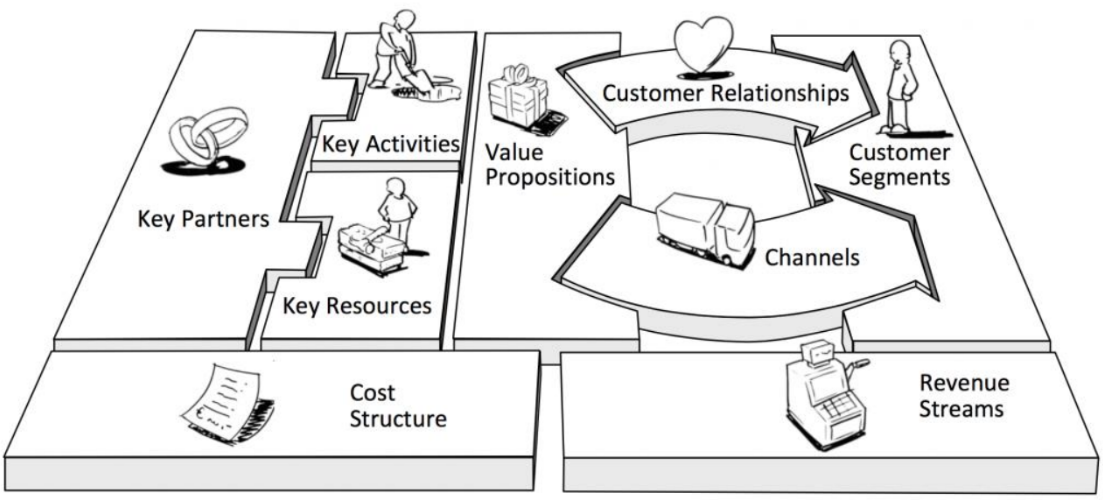
\includegraphics[width=0.7\linewidth]{images/business-model-canvas.PNG}
    \caption{Business Model Canvas}
    \label{fig:business-model-canvas}
\end{figure}

I nove blocchi del Business Model Canvas sono:
\begin{enumerate}
    \item \textit{Segmenti di clientela:} questo blocco identifica i gruppi specifici di persone o organizzazioni che l'azienda intende raggiungere e servire.
    \item \textit{Proposta di valore:} rappresenta l'insieme di prodotti e servizi che creano valore per ogni specifico segmento di clientela.
    \item \textit{Canali:} i canali indicano come l’azienda comunica con i clienti e come raggiunge i diversi segmenti per consegnare la proposta di valore.
    \item \textit{Relazioni con i clienti:} descrive il tipo di relazioni che l'azienda instaura con ciascun segmento di clientela.
    \item \textit{Flussi di ricavi:} questo blocco rappresenta i flussi di entrate che l’azienda genera da ogni segmento di clientela.
    \item \textit{Risorse chiave:} qui si descrivono gli asset essenziali per il funzionamento del modello di business.
    \item \textit{Attività chiave:} rappresenta le principali azioni che l'azienda deve compiere per far funzionare il modello di business.
    \item \textit{Partner chiave:} delinea la rete di fornitori e partner con cui l'azienda collabora per ottimizzare il modello di business.
    \item \textit{Struttura dei costi:} raccoglie tutti i costi che l'azienda deve sostenere per far funzionare il modello di business.
\end{enumerate}

\subsection*{Proposta di valore}
La \textit{proposta di valore} è il cuore del Business Model Canvas, in quanto rappresenta il pacchetto di benefici che l'azienda offre a ciascun segmento di clientela. È la ragione per cui i clienti scelgono l'azienda rispetto ai suoi concorrenti: risolve un problema o soddisfa un bisogno specifico. La proposta di valore può essere innovativa, introducendo un'offerta completamente nuova o dirompente, oppure può essere simile a prodotti già presenti sul mercato, ma con caratteristiche migliorate o elementi aggiuntivi.

Una proposta di valore efficace si distingue in modo univoco e può determinare il successo o il fallimento del modello di business. Il valore può essere creato sia in termini quantitativi (come prezzo e velocità del servizio) sia qualitativi (come il design e l’esperienza di acquisto). Alcuni esempi di elementi che contribuiscono alla creazione di valore per i clienti includono:
\begin{itemize}
    \item \textit{Novità:} soddisfare un bisogno completamente nuovo, che i clienti non percepivano prima, come nel caso di prodotti o servizi innovativi.
    \item \textit{Performance:} migliorare le prestazioni di un prodotto o servizio, per esempio aumentando la potenza di un processore o la capacità di memoria di un dispositivo.
    \item \textit{Personalizzazione:} adattare prodotti e servizi alle esigenze specifiche di clienti o segmenti, rendendoli unici.
    \item \textit{Esecuzione di un lavoro:} creare valore aiutando i clienti a portare a termine compiti specifici.
    \item \textit{Design:} offrire un design distintivo, che può essere difficile da misurare, ma che rappresenta un importante elemento di differenziazione.
    \item \textit{Brand e status:} alcuni clienti trovano valore nell'utilizzo di un marchio noto e prestigioso.
    \item \textit{Prezzo:} offrire un prodotto simile a un prezzo inferiore, soddisfacendo le esigenze dei segmenti sensibili al prezzo.
    \item \textit{Riduzione dei costi:} aiutare i clienti a ridurre i loro costi, un fattore apprezzato in molti settori.
    \item \textit{Riduzione dei rischi:} un cliente può percepire un valore aggiuntivo nell’acquisto di prodotti che riducono i rischi o le incertezze.
    \item \textit{Accessibilità:} rendere prodotti e servizi accessibili a clienti che in precedenza non ne avevano accesso, grazie a nuove tecnologie o modelli di business innovativi.
    \item \textit{Convenienza e usabilità:} creare valore rendendo i prodotti più semplici e convenienti da usare.
\end{itemize}
Nel definire la proposta di valore, è utile riflettere su alcune domande chiave:
\begin{enumerate}
    \item Perché i clienti dovrebbero scegliere il nostro prodotto o servizio?
    \item Che tipo di valore offriamo al cliente? Quali problemi stiamo aiutando a risolvere?
    \item Quali bisogni stiamo soddisfacendo? Quale combinazione di prodotti o servizi stiamo proponendo per ciascun segmento di clientela?
\end{enumerate}

\subsection*{Segmenti di clientela}
Nel Business Model Canvas, il blocco dedicato ai \textit{segmenti di clientela} descrive i diversi gruppi di persone o organizzazioni ai quali un'azienda si rivolge. I clienti rappresentano il cuore di ogni modello di business, poiché senza clienti remunerativi, nessuna azienda può sopravvivere nel lungo termine. Comprendere e segmentare i clienti in gruppi omogenei permette all'azienda di rispondere con maggiore precisione alle loro esigenze, sviluppando offerte mirate per soddisfare bisogni specifici.

Un modello di business può includere uno o più segmenti di clientela, ognuno dei quali può variare in dimensioni, preferenze e profittabilità. Definire con attenzione i segmenti di clientela è un passo strategico, poiché il business model sarà progettato attorno ai bisogni e alle caratteristiche di tali segmenti, determinando anche quali clienti servire e quali, invece, escludere. Questa segmentazione aiuta l’azienda a creare un’offerta di prodotti e servizi altamente mirata e rilevante per ogni gruppo di clienti.

Ogni gruppo di clienti costituisce un segmento separato se possiede caratteristiche che richiedono un’offerta specifica. Un segmento può essere distinto da un altro in base ai seguenti criteri:
\begin{itemize}
    \item I bisogni dei clienti richiedono e giustificano un’offerta specifica.
    \item Ciascun segmento è raggiunto attraverso canali di distribuzione diversi.
    \item Ogni segmento richiede un diverso tipo di relazione con l’azienda.
    \item La profittabilità dei segmenti varia sensibilmente.
    \item I clienti sono disposti a pagare per aspetti diversi dell’offerta.
\end{itemize}
Esistono diversi tipi di segmenti di clientela, ciascuno con caratteristiche e strategie di marketing uniche. Ecco le principali tipologie:
\begin{itemize}
    \item \textit{Mass Market (mercato di massa):} In questo tipo di mercato, l’azienda non distingue tra diversi segmenti; la proposta di valore, i canali di distribuzione e le relazioni con i clienti sono concentrati su un unico gruppo omogeneo con bisogni simili. Questo approccio è tipico del mercato dell’elettronica di consumo, come smartphone, tablet e PC, dove l’offerta si rivolge a un pubblico ampio e generalista.
    \item \textit{Niche Market (mercato di nicchia):} Questo segmento si rivolge a mercati specializzati, dove i clienti hanno esigenze molto specifiche. Le aziende che servono un mercato di nicchia, come i produttori di componenti automobilistiche, adattano la loro offerta ai bisogni particolari di quel segmento. Le relazioni, i canali e la proposta di valore sono tutti personalizzati per rispondere alle caratteristiche uniche di questa clientela.
    \item \textit{Segmented (segmentato):} In questo caso, l'azienda distingue tra segmenti di mercato in base a caratteristiche come il potere di spesa o l’uso finale del prodotto. Un esempio è un produttore di orologi che si rivolge sia a clienti che acquistano Swatch, sia a quelli che acquistano Rolex, con due proposte di valore molto differenti. Un altro esempio è un fornitore di componenti micromeccanici che serve sia il settore medico sia quello dell’automazione industriale, adattando la proposta di valore per ogni segmento in base alle esigenze specifiche.
    \item \textit{Diversified (diversificata):} Un’azienda con un approccio diversificato serve due segmenti distinti e non correlati, ognuno con bisogni e problemi differenti. Un esempio emblematico è Amazon, che oltre al marketplace offre anche servizi cloud (AWS), rivolti a una clientela completamente diversa. Questa diversificazione sfrutta la potente infrastruttura IT sviluppata inizialmente per supportare il marketplace, utilizzandola poi come base per un nuovo modello di business.
    \item \textit{Multi-sided Platforms (piattaforme multilaterali):} Questo modello di business si rivolge a segmenti interdipendenti che sono necessari per il funzionamento dell’intero ecosistema. Un esempio è quello delle carte di credito, che richiedono sia una base estesa di utenti sia un numero ampio di esercizi che le accettano come metodo di pagamento. Entrambi i segmenti devono essere presenti affinché il modello di business abbia successo.
\end{itemize}
Durante la progettazione dei segmenti di clientela, è utile porsi alcune domande strategiche:
\begin{enumerate}
    \item Per chi stiamo creando valore?
    \item Chi sono i nostri clienti più importanti?
\end{enumerate}

\subsection*{Canali}
Il blocco dei \textit{canali} descrive come un’azienda comunica e raggiunge i suoi segmenti di clientela per offrire la propria proposta di valore. Essi rappresentano i punti di contatto tra l'azienda e i clienti, svolgendo un ruolo fondamentale nell’esperienza complessiva del cliente. I canali non solo aiutano a sensibilizzare i clienti sui prodotti e servizi, ma sono anche il mezzo attraverso il quale il cliente può valutare l’offerta, effettuare acquisti e ricevere assistenza post-vendita.

Le funzioni principali dei canali includono:
\begin{itemize}
    \item Sensibilizzare i clienti sui prodotti e servizi dell'azienda.
    \item Supportare la valutazione da parte dei clienti della proposta di valore.
    \item Facilitare l'acquisto di prodotti e servizi.
    \item Offrire una proposta di valore.
    \item Fornire assistenza post-vendita.
\end{itemize}
Esistono diversi tipi di canali che operano in varie fasi. Si distinguono generalmente tra canali diretti (gestiti direttamente dall'azienda) e indiretti (gestiti da partner come grossisti o rivenditori), nonché tra canali di proprietà e canali dei partner. È importante trovare il giusto mix di canali, bilanciando i canali diretti e indiretti per soddisfare le preferenze dei clienti. I canali diretti includono le vendite tramite forza vendita, siti web e negozi propri, mentre i canali indiretti possono comprendere negozi di partner e grossisti.

Per ottimizzare l’efficacia dei canali, è utile rispondere a queste domande:
\begin{enumerate}
    \item Attraverso quali canali i nostri clienti vogliono essere raggiunti?
    \item Come stiamo raggiungendo i clienti ora e come sono integrati i nostri canali?
    \item Quali canali sono più efficaci e quali hanno i costi più contenuti?
    \item Come possiamo allineare i canali alle operazioni del cliente per migliorare l’esperienza complessiva?
\end{enumerate}

\subsection*{Relazioni con i clienti}
Il blocco delle \textit{relazioni con i clienti} esplora il tipo di relazione che un’azienda stabilisce con i propri segmenti di clientela. Le relazioni possono variare da modalità automatizzate a interazioni personali, e spesso dipendono da obiettivi specifici come acquisizione di nuovi clienti, mantenimento di quelli esistenti o incremento delle vendite.

Le relazioni con i clienti sono essenziali per modellare l’esperienza del cliente e possono includere diversi tipi di interazione:
\begin{itemize}
    \item \textit{Assistenza Personale:} una relazione diretta in cui un rappresentante aiuta il cliente durante e dopo la vendita.
    \item \textit{Assistenza Personale Dedicata:} un referente esclusivo è assegnato a un cliente, fornendo una relazione più intima e continua nel tempo.
    \item \textit{Self-service:} in questo caso, i clienti svolgono le operazioni autonomamente, senza interazione diretta.
    \item \textit{Servizi Automatizzati:} una combinazione di self-service avanzato e processi automatizzati che guidano il cliente.
    \item \textit{Comunità:} le aziende possono utilizzare le comunità online per coinvolgere i clienti e facilitare le connessioni tra di loro.
    \item \textit{Co-creazione:} alcune aziende, come Amazon con le recensioni, invitano i clienti a contribuire, creando valore per la comunità.
\end{itemize}
Alcune domande importanti per costruire relazioni efficaci includono:
\begin{enumerate}
    \item Quale tipo di relazione si aspetta ciascun segmento di clientela?
    \item Quali relazioni abbiamo instaurato e quali sono i relativi costi?
    \item Quanto sono integrate le relazioni con il resto del nostro modello di business?
\end{enumerate}

\subsection*{Flussi di ricavi}
Il blocco dei \textit{flussi dei ricavi} rappresenta le entrate generate dall’azienda in relazione a ciascun segmento di clientela. Se i clienti sono il cuore del modello di business, i flussi di ricavi ne rappresentano le arterie, poiché trasportano il valore economico indispensabile per la sostenibilità dell’azienda. Per individuare efficacemente i flussi di ricavi, è fondamentale chiedersi per quale valore specifico il cliente è disposto a pagare e in che modo è disposto a farlo. Rispondere correttamente a queste domande permette di generare entrate diversificate da ogni segmento di clientela.

Un business model può comprendere flussi di ricavi basati su transazioni una tantum (ad esempio, vendita di un prodotto) oppure su pagamenti ricorrenti (come abbonamenti a servizi). Ogni flusso di ricavi ha il proprio meccanismo di prezzo, che può variare da listini fissi a tariffe dinamiche basate su volume, aste, o negoziazioni. Di seguito vengono descritti alcuni dei principali meccanismi di generazione dei ricavi.

\begin{itemize}
    \item \textit{Vendita di un bene (Asset Sale):} rappresenta il modello più tradizionale, basato sulla vendita dei diritti di proprietà su un prodotto fisico.
    \item \textit{Tariffa d’uso (Usage Fee):} i ricavi sono generati in base all’utilizzo di un servizio in cui l’utente paga in proporzione all'utilizzo del servizio.
    \item \textit{Sottoscrizione (Subscription Fee):} consiste in un flusso di entrate continuo, derivante dalla vendita di accessi regolari a un servizio.
    \item \textit{Prestito, affitto o leasing (Lending/Renting/Leasing):} generano ricavi fornendo al cliente il diritto esclusivo di utilizzare un particolare bene per un periodo prestabilito ad un prezzo definito.
    \item \textit{Licenza (Licensing):} il cliente ottiene il diritto di utilizzare una proprietà intellettuale in cambio di un compenso. La licenza permette ai detentori dei diritti di generare dei ricavi dalla loro proprietà senza dover produrre un prodotto o commercializzare un servizio.
    \item \textit{Commissioni di intermediazione (Brokerage Fees):} in questo caso, i ricavi derivano dai servizi di intermediazione svolti dall’azienda per conto di due o più parti, come avviene per le piattaforme di vendita online che trattengono una percentuale su ogni transazione.
    \item \textit{Pubblicità (Advertising):} l’azienda ottiene ricavi consentendo la promozione di prodotti, servizi o marchi al proprio pubblico.
\end{itemize}
Per ottimizzare i flussi di ricavi, è utile riflettere su queste domande:
\begin{enumerate}
    \item Qual è il valore per cui i nostri clienti sono disposti a pagare?
    \item Per cosa stanno pagando ora e come?
    \item Quali modalità di pagamento preferiscono?
    \item Quanto contribuisce ciascun flusso di ricavi al totale?
\end{enumerate}

\subsection*{Risorse chiave}
Il blocco delle \textit{risorse chiave} descrive gli asset fondamentali che permettono all’azienda di operare con successo. Le risorse sono essenziali per creare e consegnare la proposta di valore, raggiungere i clienti, mantenere relazioni con i segmenti di clientela e generare ricavi. Le risorse chiave possono appartenere all’azienda, essere affittate o fornite da partner.

Ogni modello di business richiede risorse chiave diverse, che si suddividono in varie categorie:
\begin{enumerate}
    \item \textit{Risorse fisiche:} includono beni materiali come impianti di produzione, edifici, veicoli e macchinari. Queste risorse sono indispensabili per le aziende manifatturiere e logistiche.
    \item \textit{Risorse intellettuali:} comprendono asset immateriali quali marchi, brevetti, know-how, partnership strategiche e database di clienti. Queste risorse sono particolarmente importanti in settori ad alta intensità di conoscenza e tecnologia, poiché forniscono un vantaggio competitivo.
    \item \textit{Risorse umane:} ogni azienda necessita di capitale umano, ma per alcuni modelli di business, come quelli ad alta intensità di conoscenza o creativi, le risorse umane sono particolarmente rilevanti.
    \item \textit{Risorse finanziarie:} includono la liquidità, le linee di credito e le garanzie finanziarie. Queste risorse sono cruciali per aziende che richiedono investimenti continui o capitali per sostenere la crescita.
\end{enumerate}
Per identificare le risorse chiave, è utile considerare:
\begin{enumerate}
    \item Quali risorse sono indispensabili per la nostra proposta di valore?
    \item Quali risorse sono necessarie per gestire i canali distributivi?
    \item Che tipo di risorse servono per mantenere le relazioni con i clienti?
    \item Di quali risorse abbiamo bisogno per sostenere i flussi di ricavi?
\end{enumerate}

\subsection*{Attività chiave}
Il blocco delle \textit{attività chiave} descrive le azioni essenziali che un’azienda deve compiere per far funzionare il proprio modello di business. Ogni modello di business richiede una serie specifica di attività per operare con successo, così come accade per le risorse chiave. Le attività chiave sono necessarie per creare e offrire la proposta di valore, raggiungere i mercati, mantenere relazioni con i clienti e generare ricavi.

A seconda del tipo di business model, le attività chiave possono variare notevolmente. Per esempio, in un’azienda di software, le attività centrali saranno lo sviluppo e il miglioramento continuo del software; in un’azienda manifatturiera, invece, l’attenzione si concentrerà sulla produzione e sulla gestione della catena di fornitura.

Le principali categorie di attività chiave includono:
\begin{itemize}
    \item \textit{Produzione:} riguarda la progettazione, produzione e consegna di un prodotto in quantità significative o con una qualità superiore. È un’attività fondamentale per i business model delle imprese manifatturiere.
    \item \textit{Problem Solving:} include tutte le attività necessarie per trovare soluzioni specifiche ai problemi dei clienti. Settori come la consulenza o la sanità richiedono un focus particolare sul problem solving, sulla gestione della conoscenza e sulla formazione continua.
    \item \textit{Piattaforme/Reti:} i modelli di business basati su piattaforme, come Ebay, sono dominati da attività legate alla gestione, sviluppo e promozione della piattaforma stessa.
\end{itemize}
Per identificare le attività chiave, è utile porsi alcune domande:
\begin{enumerate}
    \item Quali attività sono essenziali per realizzare la nostra proposta di valore?
    \item Quali attività supportano i nostri canali distributivi?
    \item Quali attività sono necessarie per mantenere le relazioni con i clienti e generare ricavi?
\end{enumerate}

\subsection*{Partner chiave}
Il blocco dei \textit{partner chiave} descrive la rete di fornitori e partner strategici di cui l’azienda necessita per supportare il proprio modello di business. Le partnership possono essere cruciali per ottimizzare risorse, ridurre rischi, accedere a particolari capacità o ampliare l’offerta.

I principali tipi di partnership includono:
\begin{enumerate}
    \item \textit{Alleanze strategiche} tra aziende non concorrenti.
    \item \textit{Cooperazione:} partnership strategiche tra aziende concorrenti in settori specifici.
    \item \textit{Joint Ventures:} collaborazioni per sviluppare nuovi business.
    \item \textit{Relazioni acquirente-fornitore:} mirano a garantire forniture stabili e affidabili.
\end{enumerate}
Le motivazioni principali per sviluppare partnership sono:
\begin{itemize}
    \item \textit{Ottimizzazione ed economie di scala:} una delle forme più semplici di partnership o relazioni acquirente-fornitore è quella finalizzata all’ottimizzazione delle risorse e delle attività aziendali. È inefficiente e spesso antieconomico per un’azienda cercare di possedere o gestire internamente tutte le risorse o attività necessarie. Per questo, l’ottimizzazione e le economie di scala sono mirate a ridurre i costi, attraverso l’outsourcing e la condivisione di infrastrutture.
    \item \textit{Riduzione dei rischi e dell’incertezza:} in un ambiente competitivo e caratterizzato da incertezza, le partnership possono essere fondamentali per ridurre i rischi. È comune vedere aziende che competono in alcuni settori formare alleanze strategiche in altri ambiti.
    \item \textit{Acquisizione di particolari risorse e attività:}: poche aziende possiedono internamente tutte le risorse o svolgono tutte le attività necessarie per il proprio modello di business. Molte preferiscono aumentare le proprie capacità attraverso partnership strategiche che permettono loro di accedere a risorse specifiche, come conoscenze specialistiche, licenze o reti di clientela.
\end{itemize}
È utile riflettere su domande come:
\begin{enumerate}
    \item Chi sono i nostri partner e fornitori chiave?
    \item Quali risorse chiave otteniamo dai partner?
    \item Quali attività chiave vengono svolte dai partner?
\end{enumerate}

\subsection*{Struttura dei costi}
La \textit{struttura dei costi} descrive tutte le spese necessarie per far funzionare il modello di business. I costi nascono dalle risorse chiave, dalle attività chiave e dalle partnership chiave. Sebbene l’efficienza dei costi sia cruciale per qualsiasi modello di business, alcuni modelli enfatizzano maggiormente il contenimento dei costi, mentre altri si concentrano di più sulla creazione di valore.

I modelli di business basati sui costi si suddividono in:
\begin{enumerate}
    \item \textit{Cost-driven:} orientati alla minimizzazione dei costi ovunque possibile. Questo tipo di modello si focalizza su automatizzazione e outsourcing per mantenere i costi bassi.
    \item \textit{Value-driven:} meno attenti ai costi e più focalizzati sulla creazione di valore. Spesso, questi modelli offrono una proposta di valore premium e personalizzazioni elevate.
\end{enumerate}
Alcune caratteristiche principali della struttura dei costi includono:
\begin{itemize}
    \item \textit{Costi fissi:} spese che rimangono costanti indipendentemente dai volumi, come stipendi, affitti e costi dei macchinari.
    \item \textit{Costi variabili:} spese che variano in base ai volumi di produzione.
    \item \textit{Economie di scala:} riduzioni dei costi per unità man mano che aumentano i volumi.
    \item \textit{Economie di scopo:} vantaggi sui costi derivanti dall’ampliamento dell’ambito operativo.
\end{itemize}
Per ottimizzare la struttura dei costi, è utile considerare:
\begin{enumerate}
    \item Quali sono i costi più rilevanti per il nostro modello di business?
    \item Quali risorse chiave sono più costose?
    \item Quali attività chiave rappresentano le spese maggiori?
\end{enumerate}

\chapter{Testare le idee di business}
Molti imprenditori e innovatori si lasciano entusiasmare dalle loro idee, tanto da iniziare a svilupparle senza averle adeguatamente testate. Spesso, ciò accade perché queste idee sembrano brillanti durante le presentazioni, perfettamente logiche nei fogli di calcolo e irresistibili all'interno di un business plan. Tuttavia, quello che appare come una visione innovativa può trasformarsi in un’illusione se non supportato da evidenze concrete. Il problema più comune risiede proprio nell’avvio dell’esecuzione senza una validazione preliminare dell’idea.

La validazione è un passaggio fondamentale per evitare di sprecare tempo, risorse ed energie su progetti destinati al fallimento. Testare le idee attraverso esperimenti rapidi consente di apprendere, adattarsi e identificare eventuali lacune prima di impegnarsi completamente nell’esecuzione. L'obiettivo è ridurre l’incertezza e prendere decisioni basate su dati concreti piuttosto che su supposizioni.

Il processo di \textit{test delle idee di business} si basa sulla suddivisione dell’idea in piccole ipotesi testabili, che affrontano tre tipi principali di rischio:
\begin{enumerate}
    \item La \textit{desiderabilità} valuta se i clienti sono interessati al prodotto o servizio. Per esempio, il rischio potrebbe derivare da un mercato troppo piccolo, da un numero insufficiente di clienti interessati o dall’incapacità dell’azienda di raggiungere e mantenere i clienti target.
    \item La \textit{fattibilità} si concentra sulla possibilità di realizzare il progetto. Qui il rischio può essere rappresentato dalla mancanza di accesso a risorse chiave come tecnologie, proprietà intellettuali o partner fondamentali, oppure dall’incapacità di sviluppare le competenze necessarie per portare a termine le attività chiave.
    \item La \textit{sostenibilità} verifica se l’idea può generare entrate sufficienti. Un rischio in questo ambito potrebbe derivare dalla riluttanza dei clienti a pagare prezzi adeguati, dalla mancanza di margini sostenibili o da costi operativi troppo elevati.
\end{enumerate}
Per affrontare questi rischi, è necessario seguire un approccio sequenziale e iterativo: prima si identificano le ipotesi chiave, poi si conducono esperimenti per validarle, infine si analizzano le evidenze raccolte e si adattano le idee in base ai risultati ottenuti.

\begin{figure}[ht]
    \centering
    
\includegraphics[width=0.7\linewidth]{images/test-idea.PNG}
    \caption{Approccio per testare l'idea di business}
    \label{fig:test-idea}
\end{figure}

Il processo di test delle ipotesi si sviluppa attraverso una sequenza iterativa che collega riflessione, costruzione e apprendimento.
\begin{enumerate}
    \item Si parte dal formulare un’ipotesi chiave che rappresenti un aspetto specifico e critico dell’idea di business.
    \item A questa segue la progettazione di esperimenti concreti, come un Minimum Viable Product (MVP) o altre strategie per raccogliere dati utili a testare l’ipotesi.
    \item I dati raccolti vengono poi analizzati per produrre evidenze.
    \item Infine, si utilizzano le evidenze per apprendere e adattare l’idea, trasformandola gradualmente in un progetto più robusto e validato.
\end{enumerate}

\section{Ipotesi chiave}
Le \textit{ipotesi chiave} rappresentano i pilastri su cui si basano la proposta di valore, il modello di business e le strategie operative. Per esempio, un’ipotesi chiave potrebbe essere: "I clienti saranno disposti a pagare 50 euro al mese per questo servizio." Tuttavia, per evitare il pregiudizio della conferma, che spinge a cercare prove che supportino solo ciò che già si crede, è utile formulare ipotesi in modo neutro o addirittura negativo, oppure testare ipotesi concorrenti.

Un’ipotesi ben costruita ha tre caratteristiche principali:
\begin{enumerate}
    \item \textit{Testabilità}, cioè la possibilità di validarla o confutarla basandosi su evidenze raccolte.
    \item \textit{Precisione}, ovvero una chiara definizione di cosa si intende dimostrare, con indicazioni specifiche sul chi, cosa e quando.
    \item \textit{Discrezione}, nel senso che deve trattarsi di un aspetto isolato e distinto, evitando di mescolare troppe variabili in una singola ipotesi.
\end{enumerate}
Le ipotesi chiave sono strettamente collegate agli elementi principali del Business Model Canvas, in particolare ai rischi di desiderabilità, fattibilità e sostenibilità.
\begin{itemize}
    \item La \textit{desiderabilità} si riferisce ai segmenti di clientela, alla proposta di valore e ai canali. L’ipotesi qui è: "Il cliente vuole realmente ciò che stiamo offrendo?"
    \item La \textit{fattibilità} riguarda le risorse chiave, le attività chiave e i partner chiave. L’ipotesi diventa: "Possiamo effettivamente costruire e fornire questa proposta di valore?"
    \item La \textit{sostenibilità} tocca i flussi di ricavi e la struttura dei costi, con l’ipotesi: "Possiamo generare entrate sufficienti per coprire i costi e ottenere margini sostenibili?"
\end{itemize}

\subsection{Desiderabilità}
Le \textit{ipotesi di desiderabilità} si focalizzano sulla risposta del mercato all’idea di business. In altre parole, cercano di rispondere alla domanda: \textit{"Lo vogliono?"}. Nel Business Model Canvas, il rischio di mercato si riflette nei blocchi della proposta di valore, nei segmenti di clientela, nei canali e nelle relazioni con i clienti.

Per esempio, un’ipotesi di desiderabilità legata alla proposta di valore potrebbe essere: \textit{"Pensiamo che la nostra proposta di valore sia unica e sufficientemente attrattiva per i segmenti di mercato a cui ci rivolgiamo."} Analogamente, per i segmenti di clientela si potrebbe supporre: \textit{"Pensiamo che il segmento di clientela a cui ci rivolgiamo sia grande abbastanza da garantire la sostenibilità del business."}

Le ipotesi sui canali potrebbero invece indagare se sono stati scelti i giusti mezzi per raggiungere e acquisire i clienti. Infine, quelle relative alle relazioni con i clienti potrebbero valutare la capacità di costruire legami forti e duraturi, o la difficoltà per i clienti di passare alla concorrenza.

\subsection{Fattibilità}
Le \textit{ipotesi di fattibilità} analizzano la capacità dell’azienda di realizzare concretamente il proprio modello di business. Si collegano ai blocchi del Business Model Canvas che riguardano i partner chiave, le attività chiave e le risorse chiave, e rispondono alla domanda: \textit{"Possiamo farlo?"}.

Un esempio di ipotesi relativa alle attività chiave potrebbe essere: \textit{"Pensiamo di poter realizzare tutte le attività critiche al livello di qualità richiesto dal nostro modello di business."} Analogamente, le ipotesi sulle risorse chiave potrebbero esplorare la possibilità di acquisire le tecnologie, il personale qualificato e i fondi necessari. Infine, le ipotesi sui partner chiave potrebbero valutare la capacità di costruire alleanze strategiche per sostenere il modello di business.

\subsection{Sostenibilità}
Le \textit{ipotesi di sostenibilità} si concentrano sul rischio finanziario del modello di business e cercano di rispondere alla domanda: \textit{"Dovremmo farlo?"}. Queste ipotesi si collegano ai blocchi dei flussi di ricavi e della struttura dei costi.

Ad esempio, una tipica ipotesi sui flussi di ricavi potrebbe essere: \textit{"Pensiamo di poter convincere i nostri clienti a pagare un determinato prezzo per le nostre proposte di valore."} Per quanto riguarda i costi, si potrebbe supporre: \textit{"Pensiamo di poter mantenere i costi della nostra infrastruttura sotto controllo, generando margini di profitto sostenibili."}

\subsection{Mappatura delle ipotesi chiave}
La \textit{mappatura delle ipotesi} è uno strumento utile per identificare i rischi principali e assegnare loro la corretta priorità. Questo esercizio organizza le ipotesi lungo due assi: importanza ed evidenza.

L’asse orizzontale rappresenta le evidenze disponibili: le ipotesi vengono collocate a sinistra se esistono già dati rilevanti e osservabili, mentre vengono posizionate a destra se mancano evidenze concrete. L’asse verticale rappresenta invece l’importanza delle ipotesi: quelle critiche per il successo del business vengono posizionate in alto, mentre quelle meno rilevanti in basso.

Questa mappa consente di distinguere tra ipotesi che richiedono un immediato intervento e quelle che possono essere affrontate in un secondo momento. Per esempio:
\begin{itemize}
    \item \textit{Ipotesi importanti con evidenze:} Queste ipotesi devono essere analizzate attentamente per verificare la solidità delle evidenze. Se le evidenze sono valide, l’ipotesi può essere considerata confermata.
    \item \textit{Ipotesi importanti senza evidenze:} Queste sono le ipotesi prioritarie per la sperimentazione. È necessario progettare test rapidi per raccogliere dati e affrontare i rischi più critici del business.
    \item \textit{Ipotesi meno importanti:} Possono essere rinviate, indipendentemente dalla disponibilità di evidenze.
\end{itemize}
Le ipotesi di desiderabilità, fattibilità e sostenibilità possono essere posizionate sulla mappa per identificare le priorità di intervento.

\begin{figure}[ht]
    \centering
    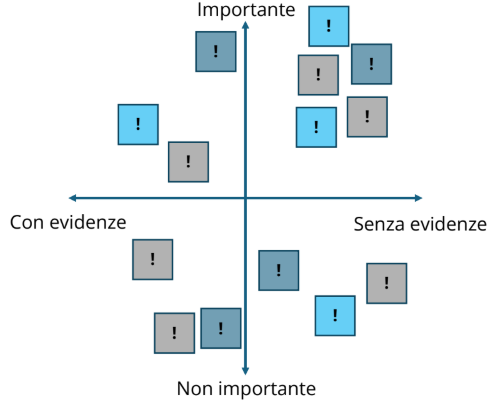
\includegraphics[width=0.5\linewidth]{images/mappa-ipotesi-chiave.PNG}
    \caption{Mappatura delle ipotesi chiave}
    \label{fig:mappa-ipotesi-chiave}
\end{figure}

\section{Esperimenti}
Gli \textit{esperimenti} sono strumenti essenziali per ridurre i rischi e le incertezze legate a un’idea imprenditoriale. Essi permettono di validare o confutare le ipotesi chiave su cui si basa un progetto, fornendo dati concreti e utili per prendere decisioni informate. Ma cosa rende un esperimento efficace?

Un esperimento ben progettato deve essere replicabile e in grado di generare dati comparabili. Questo richiede una struttura chiara, composta da quattro elementi fondamentali: un’ipotesi da testare, la definizione dell’esperimento, le metriche per misurare i risultati e i criteri di successo. Per aumentare l’affidabilità delle conclusioni, è spesso utile eseguire più esperimenti per verificare una stessa ipotesi.

\section{Evidenze}
Le \textit{evidenze} raccolte dagli esperimenti sono il fondamento per confermare o confutare le ipotesi. Possono essere ottenute attraverso dati sul campo, osservazioni dirette o comportamenti rilevati. Non tutte le evidenze, però, hanno lo stesso valore. Esse si classificano in evidenze deboli e evidenze forti, a seconda della loro affidabilità.

\begin{table}[ht]
\centering
\rowcolors{2}{lightblue}{lightgray}
\footnotesize
\begin{tabular}{|p{7cm}|p{7cm}|}
\hline
\rowcolor{headerblue}
\textbf{\textcolor{white}{Evidenze deboli}} & \textbf{\textcolor{white}{Evidenze forti}}\\\hline
\textbf{1. Opinioni (convinzioni)}\newline
Quando le persone dicono:\newline
$<<$Vorrei...$>>$; $<<$Penso che ... sia importante$>>$; $<<$Credo...$>>$ o $<<$Mi
piace$>>$
&
\textbf{1. Fatti (eventi)}\newline
Quando le persone dicono:\newline
$<<$ La scorsa settimana ...$>>$; $<<$In questa situazione in genere io
...$>>$ oppure $<<$Spendo ... in...$>>$
\\\hline
\textbf{2. Cosa dicono le persone}\newline
Cosa dicono le persone nelle interviste o nei questionari non rispecchia necessariamente cosa fanno nella vita reale o cosa faranno in futuro
&
\textbf{2. Cosa fanno le persone}\newline
Un comportamento osservabile in generale è un buon predittore di come le persone agiscono e cosa le persone potrebbero fare in futuro
\\\hline
\textbf{3. Ambientazione in laboratorio}\newline
Quando le persone sanno che si sta testando qualcosa potrebbero comportarsi diversamente rispetto alle condizioni reali
&
\textbf{3. Ambientazione nel mondo reale}\newline
Il predittore più affidabile del comportamento futuro è dato dall’osservazione delle persone quando non sanno di essere testate
\\\hline
\textbf{4. Piccoli investimenti}\newline
L'iscrizione via e-mail per essere informati sull'imminente uscita di un prodotto è un piccolo investimento e una prova di interesse relativamente debole
&
\textbf{4. Grandi investimenti}\newline
Comprare in anteprima un prodotto o la messa in gioco della propria reputazione professionale è un investimento importante e una forte prova di un reale interesse
\\\hline
\end{tabular}
\caption{Evidenze deboli e forti}
\end{table}
Questa distinzione è cruciale per decidere su quali evidenze basare le strategie aziendali. Gli esperimenti devono quindi essere progettati per raccogliere il maggior numero possibile di evidenze forti.

\section{Analizzare le evidenze}
Le evidenze da sole non bastano a ridurre i rischi di un’idea imprenditoriale; è necessario interpretarle per trarne insegnamenti. Attraverso l’analisi, si possono validare o invalidare ipotesi, scoprire nuove direzioni e prendere decisioni di business più consapevoli.

La scelta degli esperimenti da condurre dipende da diversi fattori: il tipo di ipotesi da testare, il livello di incertezza e il tempo disponibile. In generale, le regole di base prevedono di iniziare con esperimenti rapidi e a basso costo per orientarsi, per poi aumentare la complessità e l’affidabilità degli esperimenti successivi. Quando le risorse sono limitate, è essenziale scegliere l’esperimento che produce le evidenze più forti.

Gli esperimenti possono essere classificati in diverse categorie in base a obiettivi, costi e forza delle evidenze. Di seguito, alcune delle principali tipologie, organizzate in una tabella per facilitarne la consultazione.

\begin{table}[ht]
\centering
\rowcolors{2}{lightblue}{lightgray}
\footnotesize
\begin{tabular}{|p{2cm}|p{2cm}|p{2cm}|p{2cm}|p{2cm}|p{2cm}|p{2cm}|}
\hline
\rowcolor{headerblue}
\textbf{\textcolor{white}{Tipo}} & \textbf{\textcolor{white}{Esperimento}} & \textbf{\textcolor{white}{Costo}} & \textbf{\textcolor{white}{Tempo di
preparazione}} & \textbf{\textcolor{white}{Tempo di
esecuzione}} & \textbf{\textcolor{white}{Forza dell’evidenza}} & \textbf{\textcolor{white}{Rischi}}\\\hline

& Intervista con i clienti & XX & XX & XX & X & Desiderabilità e sostenibilità\\
& Intervista con esperti & XX & XX & XXX & XX & Desiderabilità e sostenibilità\\
Esplorazione & Intervista a partner e fornitori & XX & XX & XXX & XXXX & Fattibilità e sostenibilità\\
& Un giorno nella vita & XX & XX & XXX & XXX & Desiderabilità\\
& Questionario & XX & XX & XXX & X & Desiderabilità e sostenibilità\\\hline

& Analisi dei trend di ricerca & X & XX & XX & XXX & Desiderabilità e sostenibilità\\
& Analisi del traffico web & XX & XX & XXX & XX & Desiderabilità e sostenibilità\\
Analisi dati & Discussioni nei forum & X & XX & XXX & XX & Sostenibilità\\
& Riscontro forza vendita & XX & XX & XX & XX & Sostenibilità\\
& Analisi del supporto clienti & XX & XX & XXX & XX & Desiderabilità\\\hline

& Online Ad & XXX & XX & XXX & XXX & Sostenibilità\\
& Link tracking & X & X & XXX & XXX & Desiderabilità e sostenibilità\\
& 404 test & X & X & X & XXX & Desiderabilità\\
Ricerca degli interessi & Feature stub & X & XX & XX & XXXX & Desiderabilità\\
& Email campaign & X & XX & XXX & XXX & Desiderabilità e sostenibilità\\
& Social media campaign & XX & XXX & XXXXX & XXXX & Desiderabilità e sostenibilità\\
& Referral program & XXX & XX & XXXXX & XXXX & Desiderabilità e sostenibilità\\\hline

& 3D print & XXX & XXX & XX & XXX & Desiderabilità fattibilità e sostenibilità\\
& Paper prototype & X & XX & XXX & XX & Desiderabilità e sostenibilità\\
& Storyboard & XX & XX & XXX & XX & Desiderabilità e sostenibilità\\
Prototipi per la discussione & Data sheet & X & XX & XX & XX & Desiderabilità fattibilità e sostenibilità\\
& Brochure & X & XXX & XX & XXX & Desiderabilità fattibilità e sostenibilità\\
& Explainer video & XXX & XXX & XXXX & XXX & Desiderabilità e sostenibilità\\
& Boomerang & XX & XX & XX & XXX & Desiderabilità\\
& Pretend to Own & X & XX & XXXX & XX & Desiderabilità\\\hline

& Product box & XX & XX & X & XX & Desiderabilità\\
Ricerca di preferenze e priorità & Speed boat & XX & XX & X & XXX & Desiderabilità e fattibilità\\
& Card sorting & XX & XX & X & XX & Desiderabilità\\
& Buy a feature & XX & XX & X & XX & Desiderabilità fattibilità e sostenibilità\\\hline

& Clickable prototype & XX & XX & XX & XX & Desiderabilità\\
& Single feature MVP & XXXX & XXX & XXXX & XXXXX & Desiderabilità fattibilità e sostenibilità\\
Prototipi di interazione & Mash-up & XXX & XXX & XXXX & XXXXX & Desiderabilità fattibilità e sostenibilità\\
& Concierge & X & XX & XXX & XXXXX & Desiderabilità fattibilità e sostenibilità\\
& Life-sized prototype & XXXXX & XXXX & XXX & XXXXX & Desiderabilità fattibilità e sostenibilità\\\hline
\end{tabular}
\caption{Tipi di esperimenti}
\end{table}

\begin{table}[ht]
\centering
\rowcolors{2}{lightblue}{lightgray}
\footnotesize
\begin{tabular}{|p{2cm}|p{2cm}|p{2cm}|p{2cm}|p{2cm}|p{2cm}|p{2cm}|}
\hline
\rowcolor{headerblue}
\textbf{\textcolor{white}{Tipo}} & \textbf{\textcolor{white}{Esperimento}} & \textbf{\textcolor{white}{Costo}} & \textbf{\textcolor{white}{Tempo di
preparazione}} & \textbf{\textcolor{white}{Tempo di
esecuzione}} & \textbf{\textcolor{white}{Forza dell’evidenza}} & \textbf{\textcolor{white}{Rischi}}\\\hline

& Simple landing page & X & X & XXX & XX & Desiderabilità e sostenibilità\\
& Crowdfunding & XXXXX & XXXX & XXXX & XXXXX & Desiderabilità e sostenibilità\\
Call to action & Split test & XX & XX & XXX & XXX & Desiderabilità e sostenibilità\\
& Presale & XXX & XX & XXX & XXXXX & Desiderabilità e sostenibilità\\
& Validation survey & XX & XX & XXX & XX & Desiderabilità e sostenibilità\\\hline

& Wizard of Oz & XX & XXX & XXX & XXXXX & Desiderabilità fattibilità e sostenibilità\\
& Mock sale & X & X & XXX & XXX & Desiderabilità e sostenibilità\\
Simulation & Letter of intent & X & X & XX & XXX & Desiderabilità fattibilità e sostenibilità\\
& Pop-up store & XXXX & XXX & XX & XXXXX & Desiderabilità fattibilità e sostenibilità\\
& Extreme programming spike & XX & X & XX & XXXXX & Fattibilità\\\hline
\end{tabular}
\caption{Tipi di esperimenti}
\end{table}

\chapter{Value proposition}
La \textit{value proposition} è uno degli elementi fondamentali del business model canvas e del business plan. La sua importanza risiede nella capacità di sintetizzare i benefici che un prodotto o servizio può offrire ai clienti. Proprio per questa centralità, la definizione della value proposition merita un'attenzione particolare e un approfondimento metodologico.

Un modello particolarmente utile in questo contesto è il \textit{Value Proposition Canvas}, sviluppato dagli stessi autori del business model canvas. Questo strumento permette di esplorare e descrivere con precisione i bisogni dei clienti e come un prodotto o servizio possa soddisfarli.

\section{Value Proposition Canvas}
Il \textit{Value Proposition Canvas}\index{Business model!Value Proposition Canvas} (Figura \ref{fig:value-proposition-canvas}) si articola in due componenti principali:
\begin{enumerate}
    \item \textit{Il profilo del cliente (customer profile):} consente di comprendere come il cliente percepisce i propri bisogni e i risultati che desidera raggiungere.
    \item \textit{La mappa del valore (value map):} In questa parte, si descrive come il prodotto o servizio proposto mira a creare valore per il cliente, soddisfacendo le sue esigenze.
\end{enumerate}

\begin{figure}[ht]
    \centering
    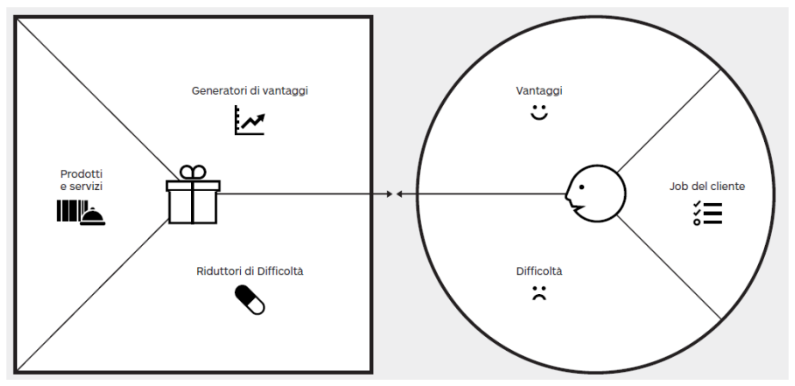
\includegraphics[width=0.7\linewidth]{images/value-proposition-canvas.PNG}
    \caption{Value Proposition Canvas}
    \label{fig:value-proposition-canvas}
\end{figure}

L’obiettivo del modello è trovare un "incastro" perfetto tra questi due elementi. Quando le caratteristiche della mappa del valore corrispondono ai bisogni espressi nel profilo del cliente, si ottiene un allineamento efficace.

Il profilo del cliente descrive dettagliatamente un segmento specifico della clientela. Il profilo si articola in tre sezioni:
\begin{itemize}
    \item \textit{Job del cliente (Customer Jobs):} ciò che i clienti vogliono ottenere, sia nel contesto lavorativo sia nella vita personale.
    \item \textit{Difficoltà (Pains):} rappresentano gli ostacoli, i rischi e i risultati negativi che il cliente affronta per raggiungere i suoi obiettivi.
    \item \textit{Vantaggi (Gains):} si riferiscono ai benefici concreti o agli obiettivi desiderati che il cliente vuole ottenere.
\end{itemize}
La value map, invece, descrive in modo dettagliato come l’azienda intende soddisfare il profilo del cliente. Anch’essa è composta da tre elementi:
\begin{itemize}
    \item \textit{Prodotti e servizi:} la lista di tutti i prodotti e servizi su cui è costruita la proposta di valore.
    \item \textit{Riduttori di difficoltà (Pain Relievers):} descrivono in che modo l’offerta proposta contribuisce a ridurre o eliminare difficoltà, rischi o insoddisfazioni del cliente.
    \item \textit{Generatori di vantaggi (Gain Creators):} aspetti che creano benefici o miglioramenti per il cliente.
\end{itemize}

\subsection{Profilo del cliente}
Per progettare una value proposition efficace, è fondamentale comprendere a fondo il cliente. L’obiettivo è mettersi nei suoi panni, cercando di visualizzare i suoi bisogni e desideri in modo chiaro e condivisibile. Questo processo culmina nella creazione di un profilo del cliente che raccoglie, in una sola pagina, elementi "azionabili", ossia utili per orientare la progettazione di prodotti e servizi.

Per iniziare, è necessario identificare un segmento specifico di clientela. Questo consente di restringere il campo e concentrarsi su un gruppo omogeneo, caratterizzato da necessità e comportamenti simili. Una volta selezionato il segmento, si passa all’identificazione dei job, delle difficoltà e dei vantaggi associati ai clienti. Questo processo deve essere completato con una priorizzazione, poiché non tutti i job, né tutte le difficoltà o i vantaggi, hanno la stessa importanza per il cliente.

\subsubsection{Job del cliente}
I job del cliente rappresentano ciò che i clienti cercano di ottenere, sia nella loro vita personale che professionale. Possono essere obiettivi concreti, problemi che desiderano risolvere o necessità che sperano di soddisfare. È fondamentale adottare il punto di vista del cliente: ciò che un'azienda considera importante potrebbe non corrispondere a ciò che il cliente percepisce come prioritario.

I job possono essere suddivisi in quattro categorie principali:
\begin{enumerate}
    \item \textit{Job funzionali}, che riguardano compiti pratici e risoluzione di problemi specifici.
    \item \textit{Job sociali}, relativi al desiderio di apparire bene agli occhi degli altri o ottenere riconoscimento sociale.
    \item \textit{Job personali o emozionali}, connessi alla ricerca di uno stato emotivo desiderato, come sentirsi sicuri, apprezzati o felici.
    \item \textit{Job di supporto}, che emergono durante l'intero ciclo di vita della value proposition. Questi includono attività legate all'acquisto, come valutare offerte o completare un ordine; alla co-creazione di valore, come fornire feedback; e alla gestione del valore a fine ciclo, come smaltire un prodotto o interrompere un abbonamento.
\end{enumerate}
Un elemento cruciale è il contesto in cui i job vengono svolti, poiché questo può influenzare le priorità e introdurre vincoli. Inoltre, non tutti i job hanno la stessa rilevanza: alcuni sono fondamentali per il cliente, mentre altri possono essere trascurati senza conseguenze significative.

Per identificare i job del cliente, è utile porsi alcune domande:
\begin{enumerate}
    \item Qual è l'unica cosa che il cliente non poteva vivere senza terminare? Quali sono i passi che potrebbero aiutare il cliente ad ottenere questo lavoro chiave?
    \item Quali sono i differenti contesti in cui potrebbero trovarsi i clienti? Come le loro attività ed obiettivi cambiano questi diversi contesti?
    \item Di cosa ha bisogno il cliente per realizzare un'interazione coinvolgente con gli altri?
    \item Quali compiti i clienti stanno cercando di fare nel loro lavoro o vita personale? Quali problemi funzionali i clienti stanno cercando di risolvere?
    \item Ritenete che ci siano problemi che i clienti hanno e che non sono nemmeno consapevoli?
    \item Quali bisogni emotivi i clienti stanno cercando di soddisfare? Che lavoro, se completato, avrebbe dato all'utente un senso di autocompiacimento?
    \item Come il cliente desidera essere percepito dagli altri? Cosa possono fare i cliente per aiutarsi ad essere percepiti in questa maniera?
    \item Come vuole sentirsi il cliente? Cosa devo fare i clienti per sentirsi in questo modo?
    \item Monitora l'interazione del cliente con un prodotto o servizio per tutta la sua durata. Quali jobs di supporto emergono nell'arco di questo ciclo di vita? L'utente cambia il suo ruolo nel corso di questo processo?
\end{enumerate}

\subsubsection{Difficoltà del cliente}
Le difficoltà dei clienti rappresentano tutti quegli ostacoli che incontrano prima, durante e dopo il tentativo di portare a termine un lavoro o "job". Possono impedire il completamento del job, renderlo più complicato o aumentarne il rischio di fallimento. Questo concetto comprende anche i rischi che derivano da un job eseguito in modo inefficace o incompleto, che possono avere ripercussioni negative significative. Possono essere di diversa natura e gravità, e comprendono:
\begin{enumerate}
    \item \textit{Risultati non desiderati, problemi e caratteristiche}.
    Queste difficoltà possono essere di natura diversa:
    \begin{itemize}
        \item \textit{Funzionali:} Ad esempio, un prodotto o servizio che non funziona come dovrebbe, non risolve il problema o ha effetti collaterali indesiderati.
    \item \textit{Sociali:} La paura di fare una brutta figura o di perdere la stima degli altri.
    \item \textit{Emozionali:} Situazioni che generano disagio, ansia o stress ogni volta che il cliente prova a completare un job.
    \item \textit{Ancillari:} Aspetti specifici di un prodotto o servizio che il cliente non gradisce, come una caratteristica non intuitiva o un'interfaccia complicata.
    \end{itemize}
    \item \textit{Ostacoli}.
    Questi sono i fattori che impediscono al cliente di iniziare un job o che ne rallentano l’esecuzione.
    \item \textit{Rischi (potenziali esiti negativi)}.
    I rischi rappresentano gli scenari in cui qualcosa può andare storto, con conseguenze significative per il cliente.
\end{enumerate}
Le difficoltà dei clienti possono essere moderate o estreme.
Per progettare soluzioni efficaci è fondamentale descrivere in modo concreto le difficoltà incontrate dai clienti e comprendere come le percepiscono. Questo processo permette di sviluppare riduttori di difficoltà mirati, ovvero soluzioni che semplificano il lavoro o eliminano gli ostacoli.

Alcune domande utili per esplorare in profondità le difficoltà dei clienti sono:
\begin{enumerate}
    \item Qual è la definizione che danno i vostri clienti di "troppo costoso"? Richiede molto tempo, costa
troppo denaro, o richiede molta fatica?
    \item Che cosa fa stare male i vostri clienti? Quali sono le loro frustrazioni, che cosa dà loro fastidio, o quali sono le cose che fanno venire loro il mal di testa?
    \item Sotto quale aspetto le proposte di valore attuali non hanno prestazioni sufficienti per i vostri clienti? Quali caratteristiche sono mancanti? Vi sono questioni di prestazioni che danno loro fastidio, parlano di malfunzionamenti?
    \item Quali sono le difficoltà e le sfide principali che i vostri clienti incontrano? Capiscono come funzionano le cose, hanno difficoltà a fare certe cose o ad affrontare jobs particolari per ragioni specifiche?
    \item Quali conseguenze sociali negative i vostri clienti incontrano o temono? Hanno paura di perdere la faccia, potere, fiducia o status?
    \item Quali rischi temono i vostri clienti? Hanno paura di rischi finanziari, sociali o tecnici, o si chiedono che cosa potrebbe andare storto?
    \item Che cosa non li fa dormire la notte? Quali sono i loro grandi problemi, le grandi preoccupazioni?
    \item Quali errori comuni commettono? Stanno usando una soluzione nel modo sbagliato?
    \item Quali barriere impediscono ai vostri clienti di adottare una proposta di valore? I costi di investimento sono elevati, la curva di apprendimento è ripida, o esistono altri ostacoli che impediscono l'adozione?
\end{enumerate}

\subsubsection{Vantaggi del cliente}
I vantaggi rappresentano i risultati e i benefici che i clienti desiderano ottenere. Questi vantaggi possono includere utilità funzionali, miglioramenti sociali, emozioni positive e risparmi su costi o risorse. Alcuni vantaggi sono esplicitamente richiesti o attesi, mentre altri possono essere desiderati o persino sorprendere piacevolmente i clienti.

I vantaggi si suddividono in quattro categorie principali, con diversi livelli di rilevanza:
\begin{enumerate}
    \item \textit{Vantaggi richiesti.}
    Questi sono i vantaggi fondamentali senza i quali una soluzione non può funzionare. Rappresentano il requisito minimo per soddisfare i clienti.
    \item \textit{Vantaggi attesi.} Questi vantaggi sono considerati standard. Sebbene una soluzione possa funzionare anche senza di essi, i clienti li danno per scontati e si aspettano di trovarli.
    \item \textit{Vantaggi desiderati.} Questi benefici superano le aspettative di base. I clienti non li considerano essenziali, ma li vorrebbero fortemente se disponibili.
    \item \textit{Vantaggi inattesi.} Questi sono vantaggi sorprendenti che vanno oltre i desideri o le aspettative dei clienti. Sono spesso un elemento di differenziazione significativa, poiché i clienti non li avrebbero nemmeno immaginati.
\end{enumerate}
I vantaggi possono essere classificati in base alla loro importanza come essenziali o nice to have. Per sviluppare soluzioni efficaci, è necessario descrivere i vantaggi in modo concreto e comprendere come i clienti li valutano. Questo permette di creare generatori di vantaggi che rafforzano la proposta di valore.

Per identificare i vantaggi del cliente, è utile considerare:
\begin{enumerate}
    \item Quali risparmi sarebbero apprezzati dai clienti?
In termini di tempo, denaro o sforzo, quali riduzioni potrebbero renderli felici?
    \item Quali livelli di qualità si aspettano i clienti? Cosa vorrebbero in quantità maggiore o minore, e quale qualità considerano indispensabile?
    \item Quali caratteristiche attuali deliziano i clienti? Ci sono elementi o funzionalità delle soluzioni attuali che i clienti trovano particolarmente utili o apprezzano?
    \item Che cosa potrebbe semplificare la vita o i jobs dei clienti? Potrebbero desiderare una curva di apprendimento più semplice, più servizi inclusi o costi di proprietà inferiori?
    \item Quali conseguenze sociali positive cercano i clienti? Vogliono rafforzare il loro status, migliorare la loro immagine o provare emozioni positive?
    \item Quali aspetti ricercano maggiormente? Sono attratti da un design eccellente, garanzie, o caratteristiche specifiche che migliorano la loro esperienza?
    \item Quali sogni o aspirazioni hanno i clienti? Quali risultati o esperienze considererebbero di grande valore o sollievo?
    \item Come misurano il successo e il fallimento? Quali metriche utilizzano per valutare la qualità, i costi e le prestazioni di una soluzione?
    \item Cosa potrebbe incentivare i clienti ad adottare una proposta di valore? Costi inferiori, minori rischi, investimenti più contenuti o qualità migliorata sono elementi che aumenterebbero la probabilità di adozione?
\end{enumerate}

\subsubsection{Classificare job, difficoltà e vantaggi}
È importante comprendere le priorità dei clienti, anche se le preferenze possono variare. Per classificare job, difficoltà e vantaggi è utile:
\begin{itemize}
    \item Identificare i job che la maggioranza considera importanti o insignificanti.
    \item Distinguere tra difficoltà percepite come estreme e quelle giudicate moderate.
    \item Determinare quali vantaggi sono essenziali e quali sono semplicemente nice to have.
\end{itemize}

\subsection{Mappa del valore}
Immaginare di calarsi nei panni dei clienti è un passaggio fondamentale per creare una proposta di valore efficace. Questo processo ha come obiettivo quello di descrivere chiaramente in che modo prodotti e servizi offerti possano generare valore per i clienti. Il risultato finale di questo lavoro dovrebbe essere una proposta di valore sintetica, organizzata in una sola pagina, ma capace di catturare l'essenza dell'offerta.

Per costruire una proposta di valore, occorre seguire alcuni passi chiave. Innanzitutto, è necessario identificare tutti i prodotti e servizi che si offrono. Successivamente, bisogna analizzare come questi riducono le difficoltà incontrate dai clienti nel raggiungere i propri obiettivi. Allo stesso modo, è fondamentale schematizzare i vantaggi che i prodotti e i servizi creano, concentrandosi su quelli che apportano benefici significativi. Infine, è importante ordinare tutte queste informazioni in base alla loro importanza per il cliente.

\subsubsection{Prodotti e i servizi}
I prodotti e i servizi costituiscono l'essenza della proposta di valore. Si tratta di ciò che l’azienda offre ai propri clienti per aiutarli a svolgere attività di natura funzionale, sociale o emotiva, o per soddisfare bisogni fondamentali. Tuttavia, è essenziale ricordare che i prodotti e i servizi non creano valore in maniera autonoma. Essi acquistano valore solo quando si riferiscono a un segmento specifico di clienti, ai loro obiettivi e alle difficoltà che incontrano.

Un’offerta può essere composta da vari tipi di prodotti e servizi:
\begin{itemize}
    \item Fisici o tangibili, come beni di consumo o prodotti manifatturieri.
    \item Intangibili, quali servizi o diritti d’autore.
    \item Digitali, come app, piattaforme o contenuti online.
    \item Finanziari, come assicurazioni, fondi di investimento o altri strumenti.
\end{itemize}

\subsubsection{Riduttori di difficoltà}
Uno degli elementi centrali di una proposta di valore sono i cosiddetti "riduttori di difficoltà". Questi descrivono in che modo i prodotti o servizi sono in grado di affrontare e risolvere le difficoltà specifiche dei clienti. Le difficoltà possono essere di vario tipo: ostacoli pratici, emotivi o logistici che impediscono ai clienti di raggiungere i loro obiettivi.

Le migliori proposte di valore non cercano di risolvere ogni singolo problema, ma si concentrano sulle difficoltà che sono davvero importanti per i clienti, in particolare quelle estreme. Ad esempio, un servizio di trasporto condiviso può ridurre le difficoltà logistiche, come il trovare un parcheggio o affrontare i costi di manutenzione di un veicolo privato.

Un aspetto cruciale è che questi riduttori non devono affrontare ogni problema individuato, ma concentrarsi su quelli che possono essere eliminati o alleviati in modo eccellente.

Per identificare i riduttori di difficoltà ci si potrebbe chiedere: I prodotti e servizi potrebbero...
\begin{enumerate}
    \item ... produrre risparmi? In termini di tempo, soldi o sforzi.
    \item ... far sentire meglio i vostri clienti? Eliminando le frustrazioni, fastidi e altre cose che fanno star male i vostri clienti.
    \item ... fissare soluzioni meno performanti? Introducendo nuove caratteristiche, prestazioni migliori o una maggiore qualità.
    \item ... porre fine alle difficoltà e alle sfide che i vostri clienti incontrano? Rendendo le cose più facili o eliminando ostacoli.
    \item ... eliminare le conseguenze sociali negative che i vostri clienti incontrano o temono? in termini di perdita di reputazione, potere, fiducia o status.
    \item ... eliminare i rischi che i vostri clienti temono? In termini di rischi finanziari, sociali, tecnici, o di cose che potrebbero andar male.
    \item ... aiutare i vostri clienti a dormire meglio la notte? Affrontando problemi significativi, riducendo o eliminando le preoccupazioni,
    \item ... limitare o sradicare gli errori comuni dei clienti? Aiutandoli a usare una soluzione nel modo giusto.
    \item ... eliminare barriere che impediscono ai clienti di adottare proposte di valore? Introducendo costi di investimento anticipato più bassi, o annullandoli, rendendo meno ripida la curva di apprendimento o eliminando altri ostacoli che impediscono l'adozione.
\end{enumerate}

\subsubsection{Generatori di vantaggi}
Un’altra componente fondamentale della proposta di valore sono i "generatori di vantaggi". Questi si riferiscono ai benefici che un prodotto o servizio può creare per i clienti, andando oltre la semplice soddisfazione delle loro necessità. Tra i vantaggi, troviamo utilità funzionale, benefici sociali, emozioni positive o risparmi economici.

Come per i riduttori di difficoltà, anche i generatori di vantaggi non devono coprire ogni singolo aspetto desiderato dai clienti. Al contrario, le proposte di valore migliori si concentrano su pochi benefici, ma lo fanno in modo eccellente.

Per identificare i generatori di vantaggi ci si potrebbe chiedere: I prodotti e servizi potrebbero...
\begin{enumerate}
    \item ... creare risparmi che farebbero piacere ai vostri clienti? In termini di tempo, denaro e fatica.
    \item ... produrre risultati che i vostri clienti si aspettano o che superano le loro aspettative? Offrendo livelli di qualità, qualcosa in più, o qualcosa in meno.
    \item ... sbaragliare le attuali proposte di valore e deliziare i vostri clienti? Riguardo a caratteristiche specifiche, prestazioni o qualità.
    \item ... rendere più facile la vita ai vostri clienti? Attraverso una migliore usabilità, accessibilità, più servizi o costi di proprietà inferiori.
    \item ... creare conseguenze sociali positive? Facendoli sentire meglio o producendo un aumento di potere o di status.
    \item ... fare qualcosa di specifico che i clienti stanno cercando? In termini di buon design, garanzie, caratteristiche specifiche o aggiuntive.
    \item ... soddisfare un desiderio, qualcosa che i clienti sognano? Aiutandoli a soddisfare le loro aspirazioni o a trovare sollievo dalle difficoltà?
    \item ... produrre risultati positivi che soddisfano i criteri di successo e fallimento dei clienti? In termini di prestazioni migliori o più a basso costo.
    \item ... contribuire a facilitare l'adozione? Attraverso il costo inferiore, meno investimenti, rischio più basso, migliore qualità, prestazioni migliorate o design migliore.
\end{enumerate}

\subsubsection{Classificare prodotti, riduttori e generatori}
Per completare la costruzione della proposta di valore, è importante classificare i prodotti, i riduttori di difficoltà e i generatori di vantaggi in base alla loro importanza. Sebbene le preferenze dei clienti possano variare, è essenziale avere un'idea chiara delle priorità più comuni. Una classificazione utile può distinguere tra ciò che è essenziale e ciò che è semplicemente "nice to have".

\section{Adeguatezza tra proposta e cliente}
Una volta completati sia il profilo cliente che la proposta di valore, il passo successivo è verificare se esiste un'adeguatezza reciproca, o "fit". Questa connessione rappresenta il momento in cui i clienti si entusiasmano per ciò che offrite. Un'adeguatezza ben riuscita si realizza quando la proposta di valore affronta un lavoro significativo per i clienti, riduce difficoltà cruciali e genera vantaggi essenziali che i clienti ritengono importanti.

In sostanza, il cliente diventa il giudice finale della proposta. Se essa non risponde pienamente ai bisogni e alle aspettative, il cliente non la accetterà, e sarà spietato nel rifiutarla. Per capire se si è raggiunta questa adeguatezza, è utile porsi due domande fondamentali: la proposta sta risolvendo le difficoltà più critiche del cliente? Sta fornendo i vantaggi che per lui sono indispensabili?

La verifica dell’adeguatezza si realizza attraverso un confronto diretto tra la proposta di valore e il profilo cliente. Questo processo consente di accertarsi che ciò che si offre risponda esattamente a ciò che interessa ai clienti.

Si parte dalla proposta di valore, analizzando uno ad uno i riduttori di difficoltà e i generatori di vantaggi. Per ogni elemento, si verifica se esso risponde ai lavori del cliente, alle sue difficoltà o ai vantaggi desiderati. Ogni elemento che si dimostra adeguato viene "spuntato" come valido. In caso contrario, se un riduttore di difficoltà o un generatore di vantaggi non è correlato a nessun bisogno del cliente, significa che non crea valore e deve essere rivisto o eliminato.

I tipi di adeguatezza da considerare sono:
\begin{enumerate}
    \item \textit{L'adeguatezza su carta:} Modello Problema-Soluzione. Questo livello di adeguatezza si concentra sulla fase di progettazione. In questo stadio, si verifica che i clienti siano effettivamente interessati a certi lavori, difficoltà e vantaggi. Successivamente, si progetta una proposta di valore che affronti direttamente questi aspetti. Questo processo avviene prevalentemente a livello teorico o concettuale, utilizzando strumenti come il Value Proposition Canvas. È il primo passo per assicurarsi che l'idea abbia un potenziale.
    \item \textit{L'adeguatezza nel mercato:} Prodotto-Mercato. A questo livello, l’obiettivo è verificare che la proposta stia creando valore reale per i clienti e stia guadagnando trazione nel mercato. Si tratta di passare dalla teoria alla pratica, osservando come i clienti utilizzano effettivamente il prodotto o servizio e quali feedback emergono.
    \item \textit{L'adeguatezza del modello di business:} Prova in banca. Infine, si verifica l’adeguatezza a livello del modello di business. Questo passaggio avviene quando si ha la conferma che la proposta di valore non solo soddisfa i clienti, ma può anche essere integrata in un modello di business profittevole e scalabile.
\end{enumerate}